\newpage

\section*{Anhang}
  \addcontentsline{toc}
    {section}
    {Anhang}



\subsection*{Elektronischer Anhang}\label{elect-anhang}
\addcontentsline{toc}
{subsection}
{Elektronischer Anhang}

Diese Dokumentation wurde zusammen mit einem elektronischen Anhang in Form einer ZIP-Datei abgegeben. Darin befinden sich der Simulator Programmiercode inklusive dessen Ergebnisse und die erstellten CAD Dateien.

\newpage
\subfile{parts/x-projektplanung}
\newpage

%%%%%%%%%%%%%%%%%% Aufgabenstellung

\subsection*{Originale Aufgabenstellung}\label{aufgabenstellung}
\addcontentsline{toc}
{subsection}
{Originale Aufgabenstellung}

Nachfolgend ist die originale Aufgabenstellung angehängt.

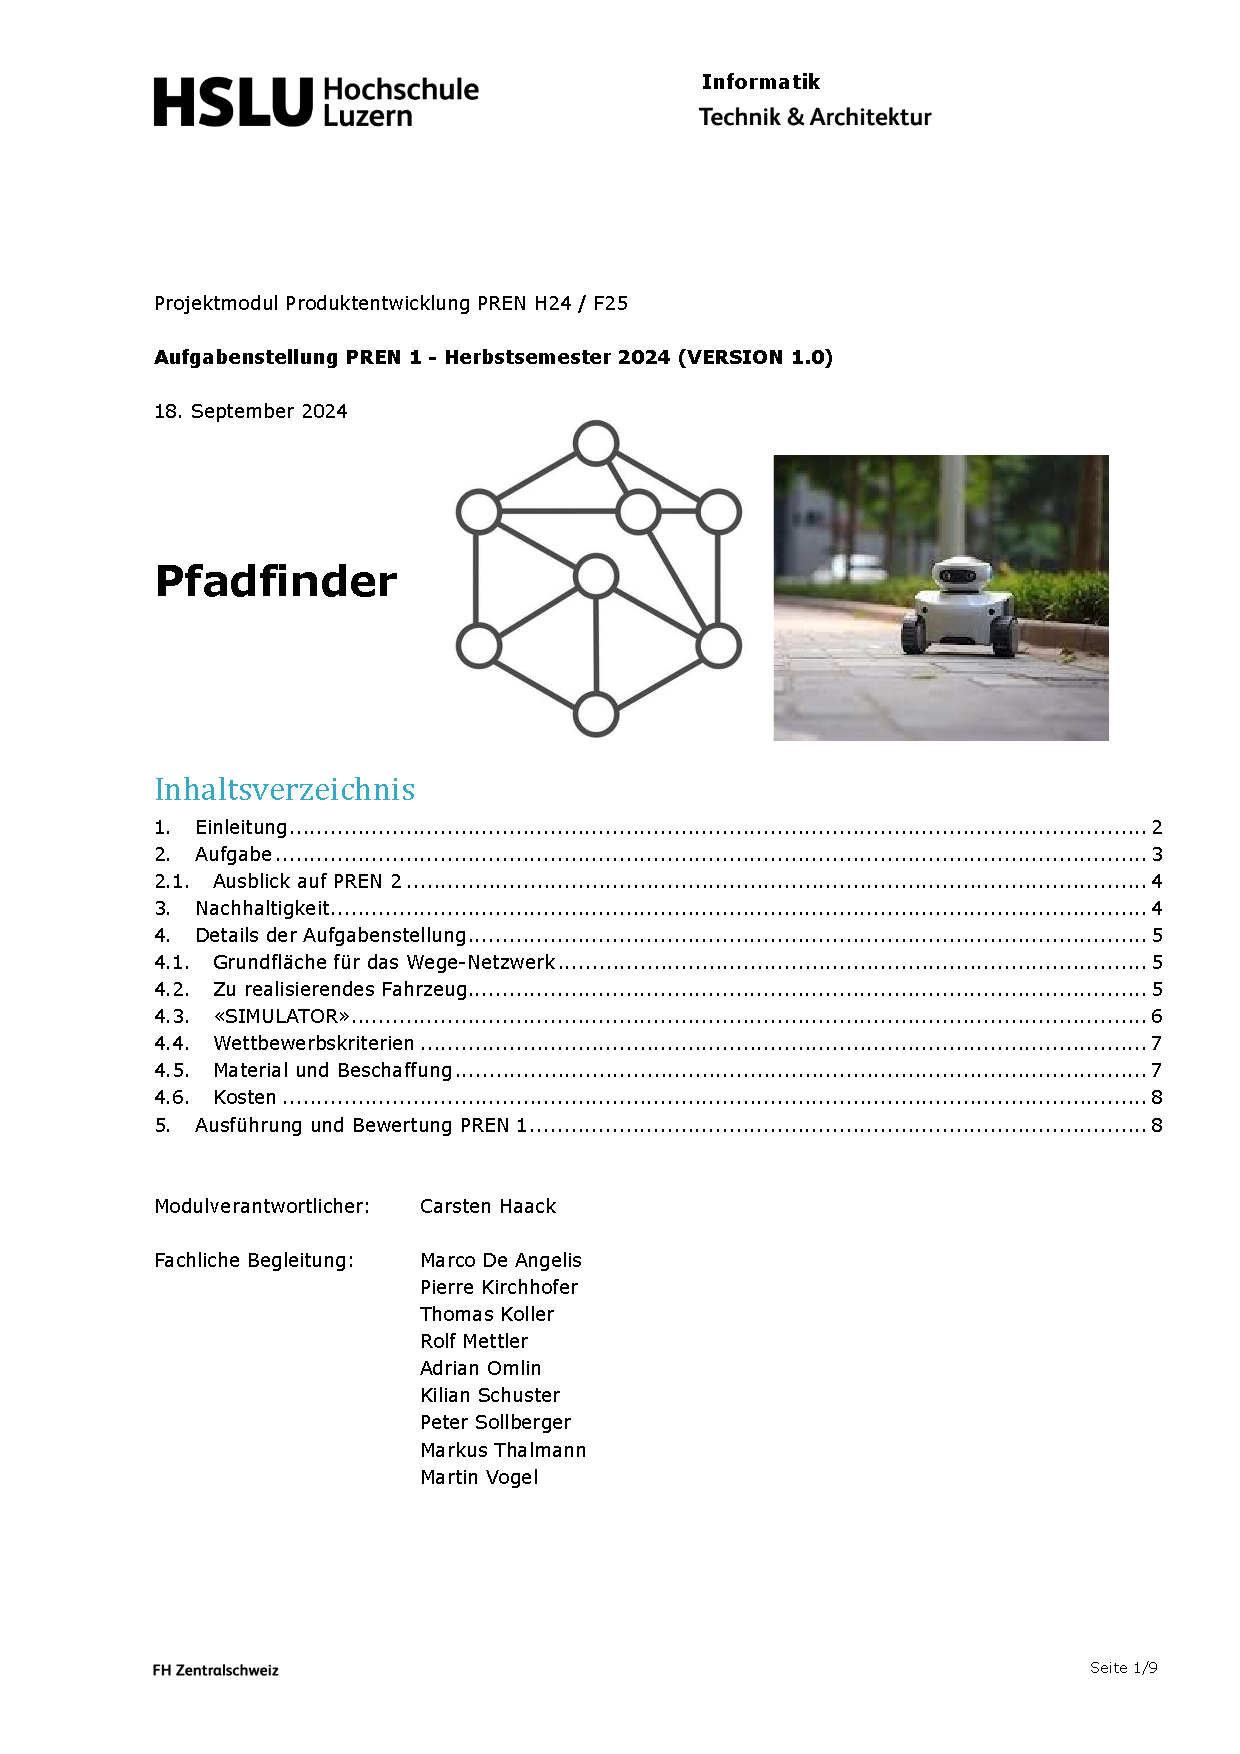
\includepdf[pages=-]{assets/projektmanagement/AufgabenstellungPREN1HS24.pdf}

%%%%%%%%%%%%%%% Anforderungsliste %%%%%%%%%%%%%%%%%%%%%%%%%

\subsection*{Anforderungsliste}\label{anforderungliste}
  \addcontentsline{toc}
    {subsection}
    {Anforderungsliste}
Die  Anforderungsliste ist ersichtlich in Tabellen \ref{table:anforderungsliste_page1} und \ref{table:anforderungsliste_page2}.

\begin{table}[H]
\centering
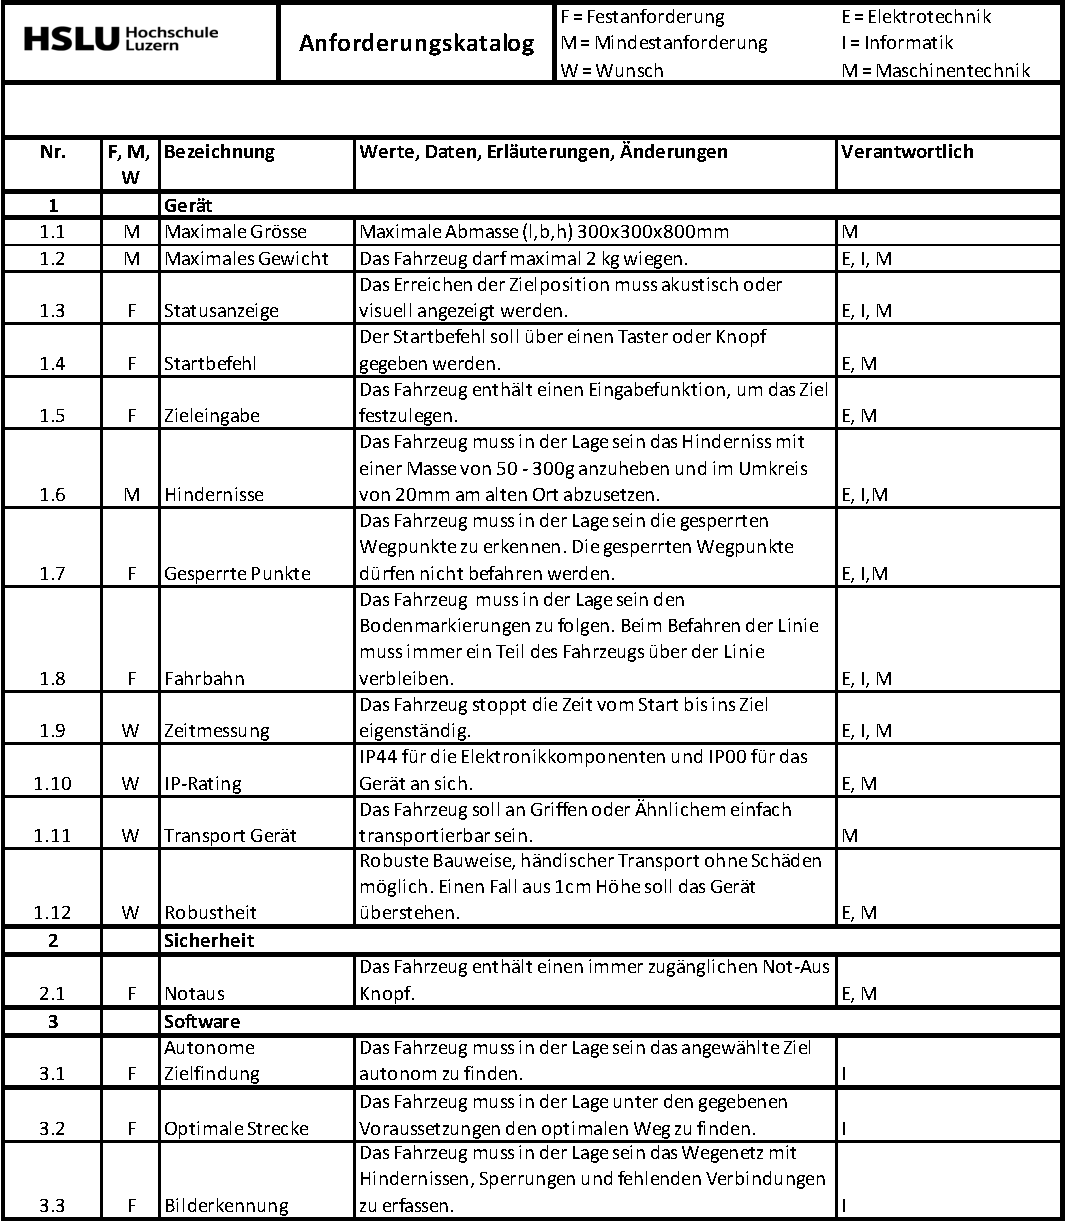
\includegraphics[width=\textwidth]{assets/projektmanagement/Anforderungsliste_V1.01_page1.pdf}
\caption{Anforderungsliste Teil 1}
\label{table:anforderungsliste_page1}
\end{table}
\newpage

\begin{table}[H]
\centering
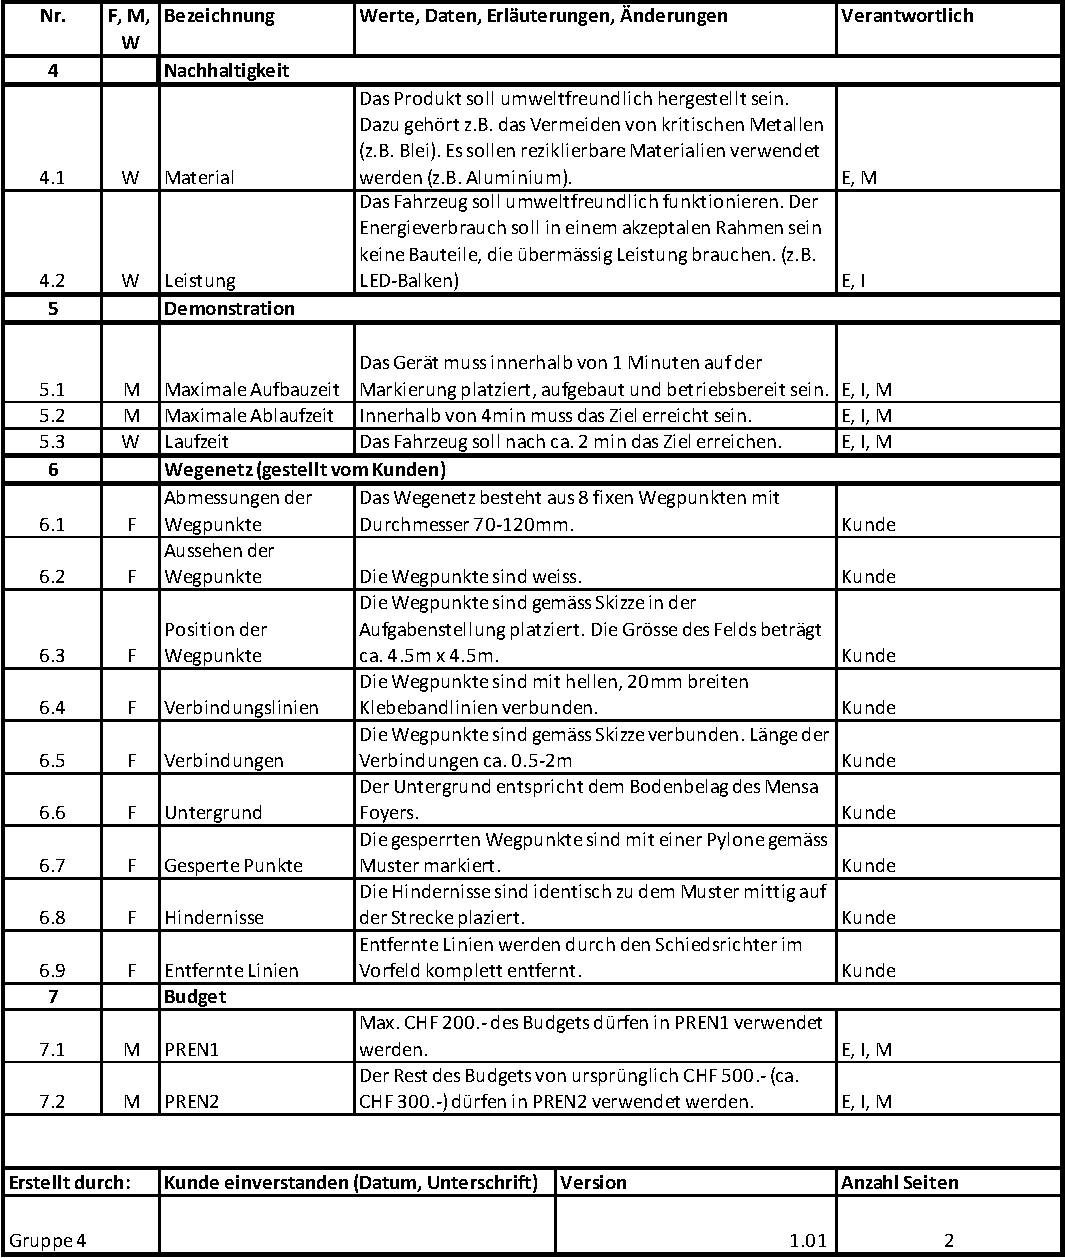
\includegraphics[width=\textwidth]{assets/projektmanagement/Anforderungsliste_V1.01_page2.pdf}
\caption{Anforderungsliste Teil 2}
\label{table:anforderungsliste_page2}
\end{table}
\newpage


%%%%%%%%%%%%%%%% Model Evaluation %%%%%%%%%%%%%%%%%%%%%%%%%5

\subsection*{YOLOv11 Model Evaluation}\label{model-evaluation}
  \addcontentsline{toc}
    {subsection}
    {YOLOv11 Model Evaluation}

Damit Pylonen, Barrieren und Knoten erkannt werden koennen, wird ein Model trainiert. Insgesamt wurden ueber 30 verschiedene YOLO Models trainiert. Viele davon wurden bereits in einem vorherigen Schritt aussortiert, da einige sehr offensichtlich schlechte Performance aufwiesen aufgrund davon, wie es die Objekte erkannt, beziehungsweise nicht erkannt hat. Auf der folgenden Seite ist eine Tabelle angehaent, in der die relevanten Models miteinander verglichen werden und das beste Model gewaehlt wurde.

Die Model Performance wird an folgenden Parametern gemessen:\cite{model-performance}

\begin{itemize}
    \item Confusion Matrix: Zeigt was das Model vorhergesagt hat und was tatsaechlich zu sehen war. Je 'diagonaler' die Matrix, desto besser.
    \item F1-Confidence: Zeigt die Balance zwischen Confidence (Wahrscheinlichkeit, dass Vorrausgesagtes stimmt) und F1 Score (Harmonischer Durchschnitt von Recall und Precision). Je hoeher der F1 Wert, desto besser.
    \item Precision-Confidence: Zeigt die Balance zwischen Precision (Anteil von 'True Positives'; wenn Model sagt, es gibt einen Knoten, wie akkurat ist diese Deutung?) und Confidence. Je tiefer die Confidence, desto besser, da dadurch der hoechste Praezisionswert bereits bei einer tieferen Confidence erreicht wird.
    \item Precision-Recall: Zeigt die Balance zwischen Precision und Recall (Faehigkeit, alle Instanzen zu erkennen). Je hoeher die Precision, desto besser.
    \item Recall-Confidence: Zeigt die Balance zwischen Recall und Confidence. Je hoeher der Recall, desto besser.
    \item Lernverlauf: Zeigt inwiefern der Verlust (Unterschied zwischen Vorhergsagtem und Realitaet) sinkt bei den Trainingsdaten und den Validationsdaten. Beginnt der Verlust bei der Validation zu steigen, deutet dies auf Overfitting hin\footnote{https://developers.google.com/machine-learning/crash-course/overfitting/overfitting}. Sollte exponentiell sinken. Zeigt, wie das Model and Wissen gewinnt. Sollte expontentiell steigen.
\end{itemize}


Der Vergleich zwischen mehreren potentiellen Modellen ist in folgendem Dokument ersichtlich. Zwei Modelle wurden jeweils verglichen aufgrund von mehreren Werten. Ist der jeweilige Wert des einen Models besser, wird diese Zelle gruen eingefaerbt.

Es wurde untersucht, ob das Modell bessere Ergebnisse bringt, wenn die beiden Barrieren pro Farbe in einzelnen Klassen aufgeteilt werden oder nicht und verschiedene Augmentationen wurden verglichen. Augmentationen werden auf die Trainingsbilder angewandt, damit diese diverser sind und zum einen mehr der Realitaet entsprechen und auch um mehr Trainingsmaterial zu haben. Ebenfalls wurde experimentiert mit unterschiedlichen Groessen der Bilder. 

\includepdf[pages=-]{assets/IT/testing/yolo/ModelComparison.pdf}


%%%%%%%%%%%%%%%%%%%%%%%%%%%target node%%%%%%%%%%%%%%%%%%%%%%%%%%%%%

\subsection*{Zielknotenerkennung}\label{target-node-unittests}
  \addcontentsline{toc}
    {subsection}
    {Zielknotenerkennung}

Die Tests der Zielknotenerkennung haben zwei Ziele:

\begin{enumerate}
    \item Parameter tunen.
    \item Funktionalitaet testen.
\end{enumerate}

\textbf{Parameter tunen}

Die Zielknotenerkennung hat folgende Parameter, deren Werte durch Tests getuned wurden. Ein Match bezeichnet einen gefundenen Erkennungspunkt des Buchstabens. Auf dem folgenden Bild \ref{img:orb-example} gibt es beispielsweise 14 Matches (Linien), deren Durchschnittliche Distanz 0 ist, da es sich um das selbe Bild handelt. Die Erkennungspunkte sind im Bild links gleich weit voneinander entfernt wie im rechten.

\begin{figure}[H]
\centering
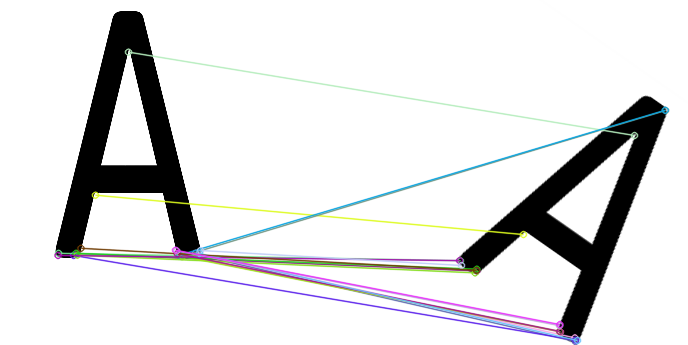
\includegraphics[width=5cm]{assets/IT/testing/target_node/orb-a.png}
\caption{Beispielbild mit Erkennungspunkten 'Matches'}
\label{img:orb-example}
\end{figure}

\begin{enumerate}
    \item MIN\_MATCHES\_REQUIRED = 10: Wie viele Matches muss es geben?
    \item MAX\_DISTANCE\_ALLOWED = 50: Wie ungenau duerfen die Matches maximal sein?
    \item Differenz Messpunkte < 5: Differenz der Anzahl Matches fuer jeden Buchstaben, um die Buchstaben mit den zwei meisten Matches vergleichen zu muessen, anstatt direkt den Buchstaben mit den meisten Matches zu nehmen.
    \item Distanz der Distanz > 5: Differenz in der durchschnittlichen Distanz der Matches der zwei Buchstaben mit den meisten Matches. Hat der Buchstaben mit weniger Matches eine Distanz, die mindestens 6 kleiner ist, passt dieser besser.
\end{enumerate}

Die finalen Werte wurden mithilfe von diesen Testresultaten in Tabelle \ref{letter-matches-orb} ermittelt. Ist die Anzahl Match Differenz grösser als 5, wird die Distanz von zwei Buchstaben gemessen.  Ist die Differenze der Distanzen grösser als 5, wird der zweite Buchstabe genommen. Werden benötigte Anzahl Matches nicht erreicht oder with die maximale Distanz überschritten, wird kein Buchstabe erkannt.

\begin{table}[H]
\centering
\small
\begin{tabularx}{\textwidth}{|c|X|X|c|X|c|}
\hline
\textbf{Buchstabe} & \textbf{Anzahl Matches pro Buchstabe} & \textbf{Anzahl Match Differenz} & \textbf{Distanz} & \textbf{Differenz Distanz} \\
\hline
None & {'A': 5, 'B': 5, 'C': 5} & 0 &  &  \\
\hline
A & {'A': 135, 'B': 42, 'C': 22} & 93 & A: 0.00 &  \\
\hline
B & {'B': 221, 'C': 51, 'A': 42} & 170 & B: 0.00 &  \\
\hline
C & {'C': 173, 'B': 51, 'A': 22} & 122 & C: 0.00 &  \\
\hline
None & {'B': 11, 'A': 10, 'C': 10} & 1 & B: 72.45, A: 63.30 & \textit{Differenzen > 50}\\
\hline
A & {'A': 21, 'B': 11, 'C': 9} & 10 & A: 18.80 &  \\
\hline
B & {'B': 25, 'A': 12, 'C': 10} & 13 & B: 13.80 &  \\
\hline
B & {'B': 28, 'A': 21, 'C': 15} & 7 & B: 15.70 &  \\
\hline
C & {'A': 24, 'C': 23, 'B': 18} & 1 & A: 45.58, C: 32.61 & 12.97 \\
\hline
C & {'B': 22, 'C': 22, 'A': 13} & 0 & B: 35.41, C: 29.77 & 5.64 \\
\hline
C & {'B': 19, 'C': 15, 'A': 13} & 4 & B: 23.30, c: 29.01 & 5.71 \\
\hline
A & {'A': 26, 'C': 14, 'B': 12} & 12 & A: 22.30 &  \\
\hline
A & {'A': 20, 'B': 13, 'C': 9} & 7 & A: 16.30 &  \\
\hline
A & {'A': 24, 'B': 12, 'C': 10} & 12 & A: 16.10 &  \\
\hline
B & {'B': 28, 'A': 22, 'C': 15} & 6 & B: 15.80 &  \\
\hline
\end{tabularx}
\caption{Analyse der Buchstaben-Matches mit Distanzen}
\label{letter-matches-orb}
\end{table}

\textbf{Funktionalitaet testen}

Die Logik, um den richtigen Buchstaben zu erkennen beschraenkt sich nicht nur auf den \acrshort{orb} Algorithmus. Es wurde selber noch ein Algorithmus implementiert. Grundsaetzlich wird der Buchstabe, fuer den die meisten Matches gefunden wurden, zurueckgeben. Jedoch ist es vor allem bei dem Buchstaben C so, dass es relativ wenige Messpunkte gibt, da der Buchstaben sehr simpel ist. Das heisst, wenn C erkannt werden soll, gibt es oft falsche Buchstaben, mit mehr Messpunkten. Falls die Buchstaben mit den meisten und den zweitmeisten Messpunkten nur 5 Messpunkte auseinander liegen, werden die Distanzen der Messpunkte verglichen. Wenn der Buchstaben, der maximal 5 Messpunkte weniger hat, eine durchschnittliche Distanz von mehr als 5 hat, wird der Buchstaben zurueckgegeben, mit den wenigeren Messpunkten. Diese Logik wird in den Unittests getestet.

Die folgenden Fälle wurden getestet:

\begin{enumerate}
    \item Buchstabe A ist ersichtlich (verschiedene Rotationen): Optimale Verhältnisse \& realistische Verhältnisse.
    \item Buchstabe B ist ersichtlich (verschiedene Rotationen): Optimale Verhältnisse \& realistische Verhältnisse.
    \item Buchstabe C ist ersichtlich (verschiedene Rotationen): Optimale Verhältnisse \& realistische Verhältnisse.
    \item Kein Buchstabe ist ersichtlich: Optimale Verhältnisse \& realistische Verhältnisse.
\end{enumerate}

\begin{table}[H]
\centering
\small
\begin{tabularx}\textwidth{ |c |X |  X | c | }
\hline
 \textbf{Bild} & \textbf{Soll} & \textbf{Ist} & \textbf{Resultat} \\
  
  \hline

       
\begin{minipage}{.1\textwidth}

\includegraphics[width=\linewidth]{assets/IT/testing/target_node/empty-node.png}
\end{minipage}
        &Kein Buchstabe erkannt.&Kein Buchstabe erkannt.&Erfüllt\\

        \hline

        
       
\begin{minipage}{.1\textwidth}

\includegraphics[width=\linewidth]{assets/IT/testing/target_node/letter-A.png}
\end{minipage}
        &Buchstabe A erkannt.&Buchstabe A erkannt.&Erfüllt\\

        \hline


        
       
\begin{minipage}{.1\textwidth}

\includegraphics[width=\linewidth]{assets/IT/testing/target_node/letter-B.png}
\end{minipage}
        &Buchstabe B erkannt.&Buchstabe B erkannt.&Erfüllt\\

        \hline

        
       
\begin{minipage}{.1\textwidth}

\includegraphics[width=\linewidth]{assets/IT/testing/target_node/letter-C.png}
\end{minipage}
        &Buchstabe C erkannt.&Buchstabe C erkannt.&Erfüllt\\

        \hline

\begin{minipage}{.1\textwidth}
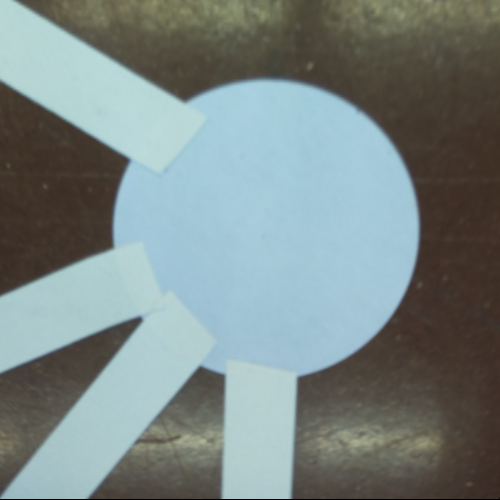
\includegraphics[width=\linewidth]{assets/IT/testing/target_node/node_after_transformation.png}
\end{minipage}
        &Kein Buchstabe erkannt.&Kein Buchstabe erkannt.&Erfüllt\\
        \hline
\begin{minipage}{.1\textwidth}
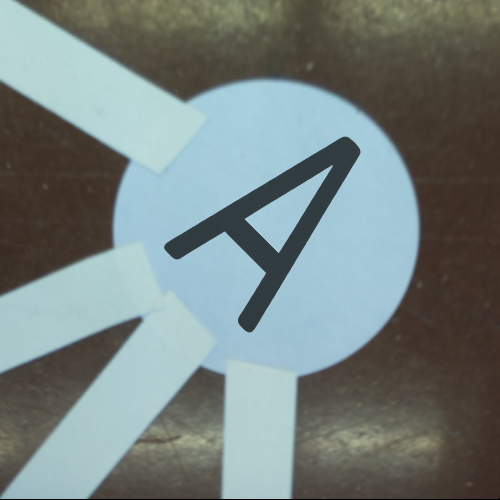
\includegraphics[width=\linewidth]{assets/IT/testing/target_node/real-a.png}
\end{minipage}
        &Buchstabe A erkannt.&Buchstabe A erkannt.&Erfüllt\\

  \hline
\begin{minipage}{.1\textwidth}
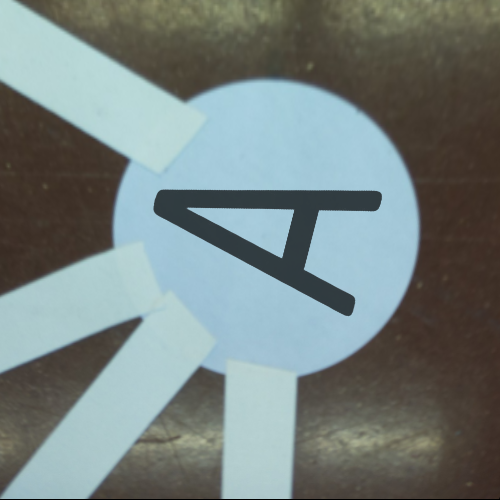
\includegraphics[width=\linewidth]{assets/IT/testing/target_node/real-a2.png}
\end{minipage}
        &Buchstabe A erkannt.&Buchstabe A erkannt.&Erfüllt\\

  \hline
\begin{minipage}{.1\textwidth}
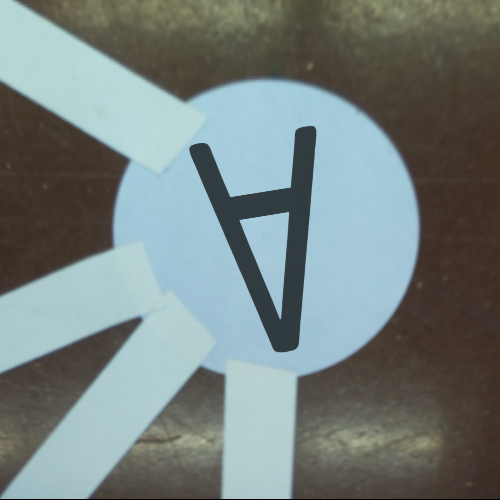
\includegraphics[width=\linewidth]{assets/IT/testing/target_node/real-a3.png}
\end{minipage}
        &Buchstabe A erkannt.&Buchstabe A erkannt.&Erfüllt\\

  \hline

  \begin{minipage}{.1\textwidth}
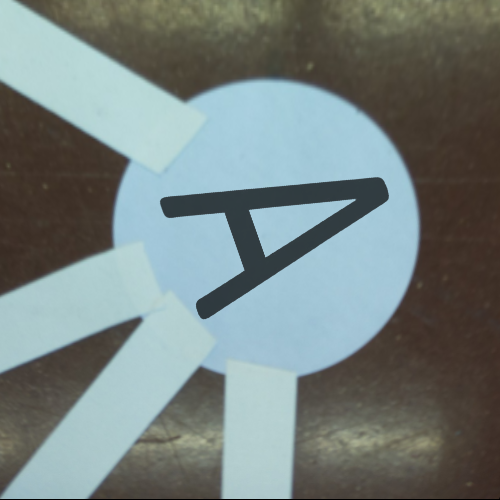
\includegraphics[width=\linewidth]{assets/IT/testing/target_node/real-a4.png}
\end{minipage}
        &Buchstabe A erkannt.&Buchstabe A erkannt.&Erfüllt\\
        \hline

  \begin{minipage}{.1\textwidth}
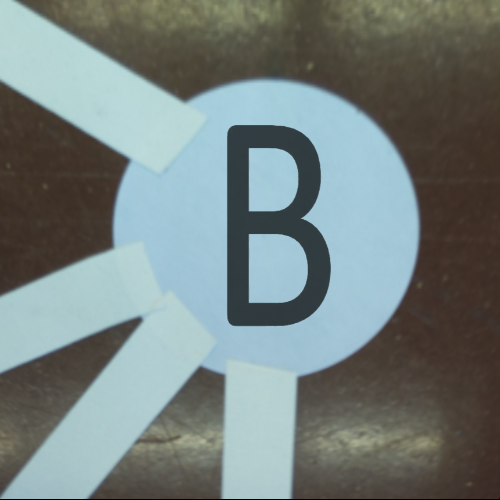
\includegraphics[width=\linewidth]{assets/IT/testing/target_node/real-b.png}
\end{minipage}
        &Buchstabe B erkannt.&Buchstabe B erkannt.&Erfüllt\\
        \hline
          \begin{minipage}{.1\textwidth}
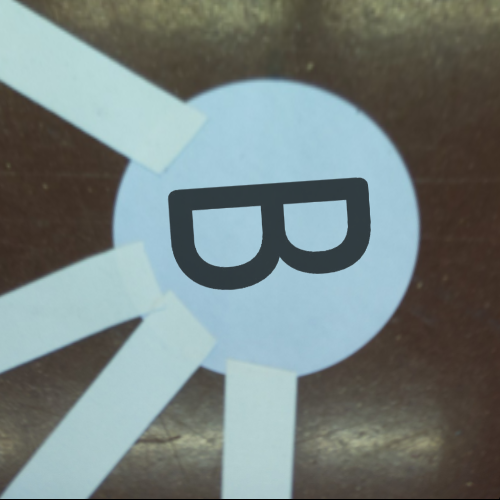
\includegraphics[width=\linewidth]{assets/IT/testing/target_node/real-b2.png}
\end{minipage}
        &Buchstabe B erkannt.&Buchstabe B erkannt.&Erfüllt\\
        \hline
          \begin{minipage}{.1\textwidth}
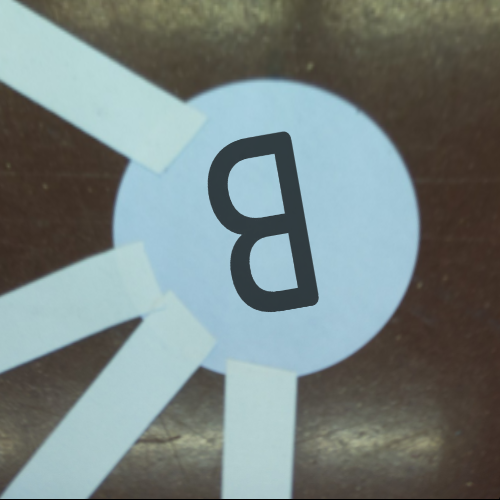
\includegraphics[width=\linewidth]{assets/IT/testing/target_node/real-b3.png}
\end{minipage}
        &Buchstabe B erkannt.&Buchstabe B erkannt.&Erfüllt\\
        \hline
         \end{tabularx}
\end{table}

\newpage

\begin{table}[H]
\centering
\small
\begin{tabularx}\textwidth{| c |X | X | c | }
\hline
 \textbf{Bild} & \textbf{Soll} & \textbf{Ist} & \textbf{Resultat} \\
  
  \hline
          \begin{minipage}{.1\textwidth}
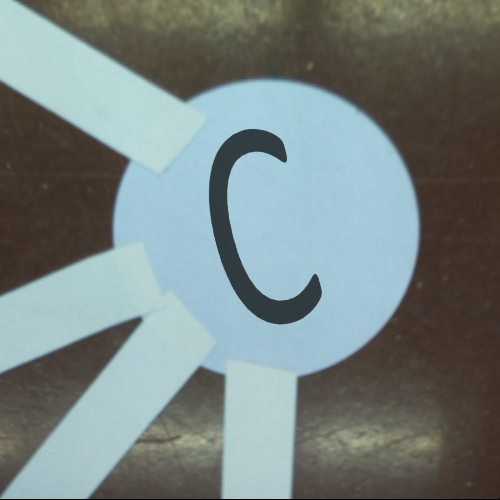
\includegraphics[width=\linewidth]{assets/IT/testing/target_node/real-c.png}
\end{minipage}
        &Buchstabe C erkannt.&Buchstabe C erkannt.&Erfüllt\\

  \hline

            \begin{minipage}{.1\textwidth}
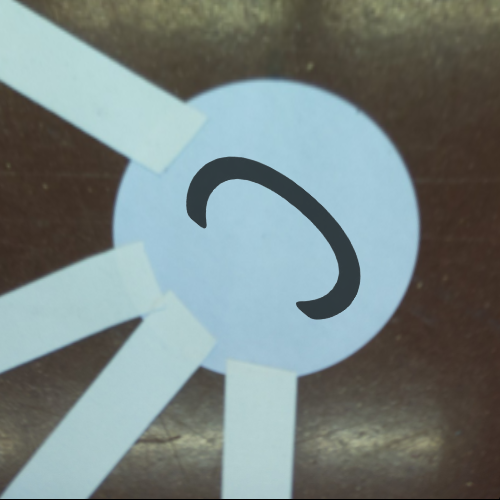
\includegraphics[width=\linewidth]{assets/IT/testing/target_node/real-c2.png}
\end{minipage}
        &Buchstabe C erkannt.&Buchstabe C erkannt.&Erfüllt\\

  \hline

            \begin{minipage}{.1\textwidth}
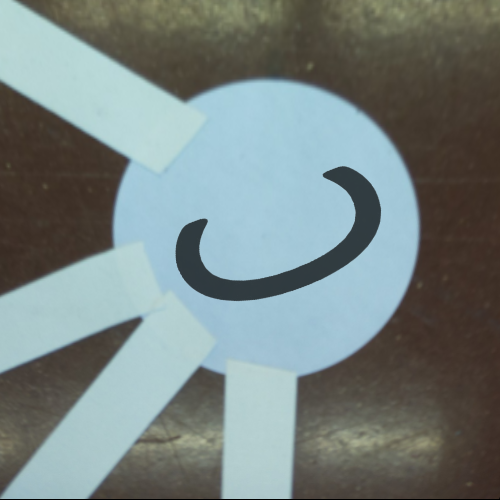
\includegraphics[width=\linewidth]{assets/IT/testing/target_node/real-c3.png}
\end{minipage}
        &Buchstabe C erkannt.&Buchstabe C erkannt.&Erfüllt\\

  \hline
\end{tabularx}
\caption{Target Node Recognition Testprotokoll}
\label{table:target-node-test}
\end{table}



Auf dem folgenden Bild \ref{img:target_node_unittests} sind alle Unittests ersichtlich, die alle erfolgreich waren.

\begin{figure}[H]
\centering
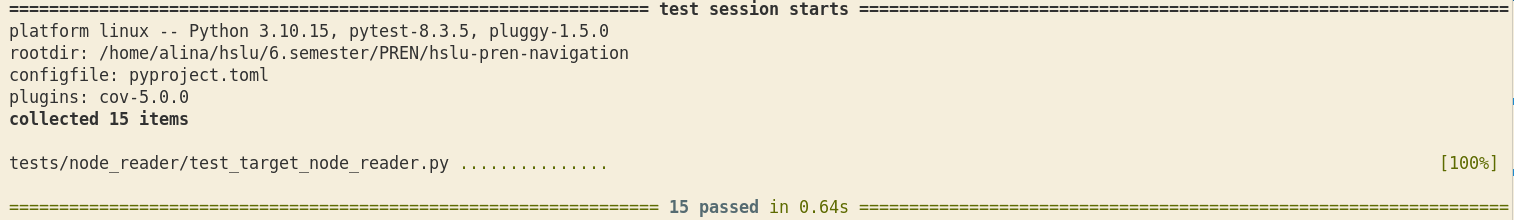
\includegraphics[width=\textwidth]{assets/IT/testing/target_node/target_node_reader_unittests.png}
\caption{Alle Target Node Unittests}
\label{img:target_node_unittests}
\end{figure}

%%%%%%%%%%%%%%%%%%%%%%%%%%%% Unittests %%%%%%%%%%%%%%%%%%%%%%%%%%%
\newpage
\subsection*{Navigation automatisierte Unittests}\label{nav-unittests}
  \addcontentsline{toc}
    {subsection}
    {Navigation automatisierte Unittests}

TODO ADD FOR EACH MODULE THAT WE HAVE, SHOW IMAGES WHERE WE USE IMAGES



\newpage
\subsubsection*{Object Detector}\label{object-detector-unittests}
\addcontentsline{toc}
{subsubsection}
{Object Detector}

Der Object Detector erhaelt Bilder und detektiert, welche Objekte sich darauf befinden mit dem YOLO Model. Dann wird ein Algorithmus angewandt, um sicherzustellen, dass nur das Objekt direkt vor dem Roboter beachtet wird, ausser hinter dem Hindernis befindet sich eine Pylone, dann soll die Pylone beachtet werden.
Die Unittests des Object Detectors sollen nicht primaer das Modell testen, sondern den Algorithmus, der das relevante Objekt findet. Folgende Szenarien wurden getestet:

\begin{enumerate}
    \item Eine Barriere befindet sich vor dem Roboter, dahinter ein Knoten.
    \item Nur ein Knoten befindet sich vor dem Roboter.
    \item Nur eine Pylone befindet sich vor dem Roboter (auf dem naechsten Knoten).
    \item Eine Barriere befindet sich vor dem Roboter, dahiner eine Pylone.
    \item Eine Barriere befindet sich vor dem Roboter, dahinter ein Knoten. Ebenfalls ist auf dem Bild eine Barriere, die nicht direkt vor dem Roboter ist.
    \item Ein Knoten befindet sich vor dem Roboter. Auf der Linie zu der Seite, befindet sich eine Barriere, die nicht vor dem Roboter ist.
\end{enumerate}

\textit{Die annotierten Bilder in der folgenden Tabelle \ref{table:object-det-test}, wurden von dem Object Detector selber annotiert in dem jeweiligen Testfall.}

\begin{table}[H]
\centering
\small
\begin{tabularx}\textwidth{|c | X |X | X | X | c | }
\hline
  \textbf{Nr} & \textbf{Bild} & \textbf{Annotiertes Bild} &\textbf{Soll} & \textbf{Ist} & \textbf{Resultat} \\
  
  \hline

        1&
\begin{minipage}{.18\textwidth}
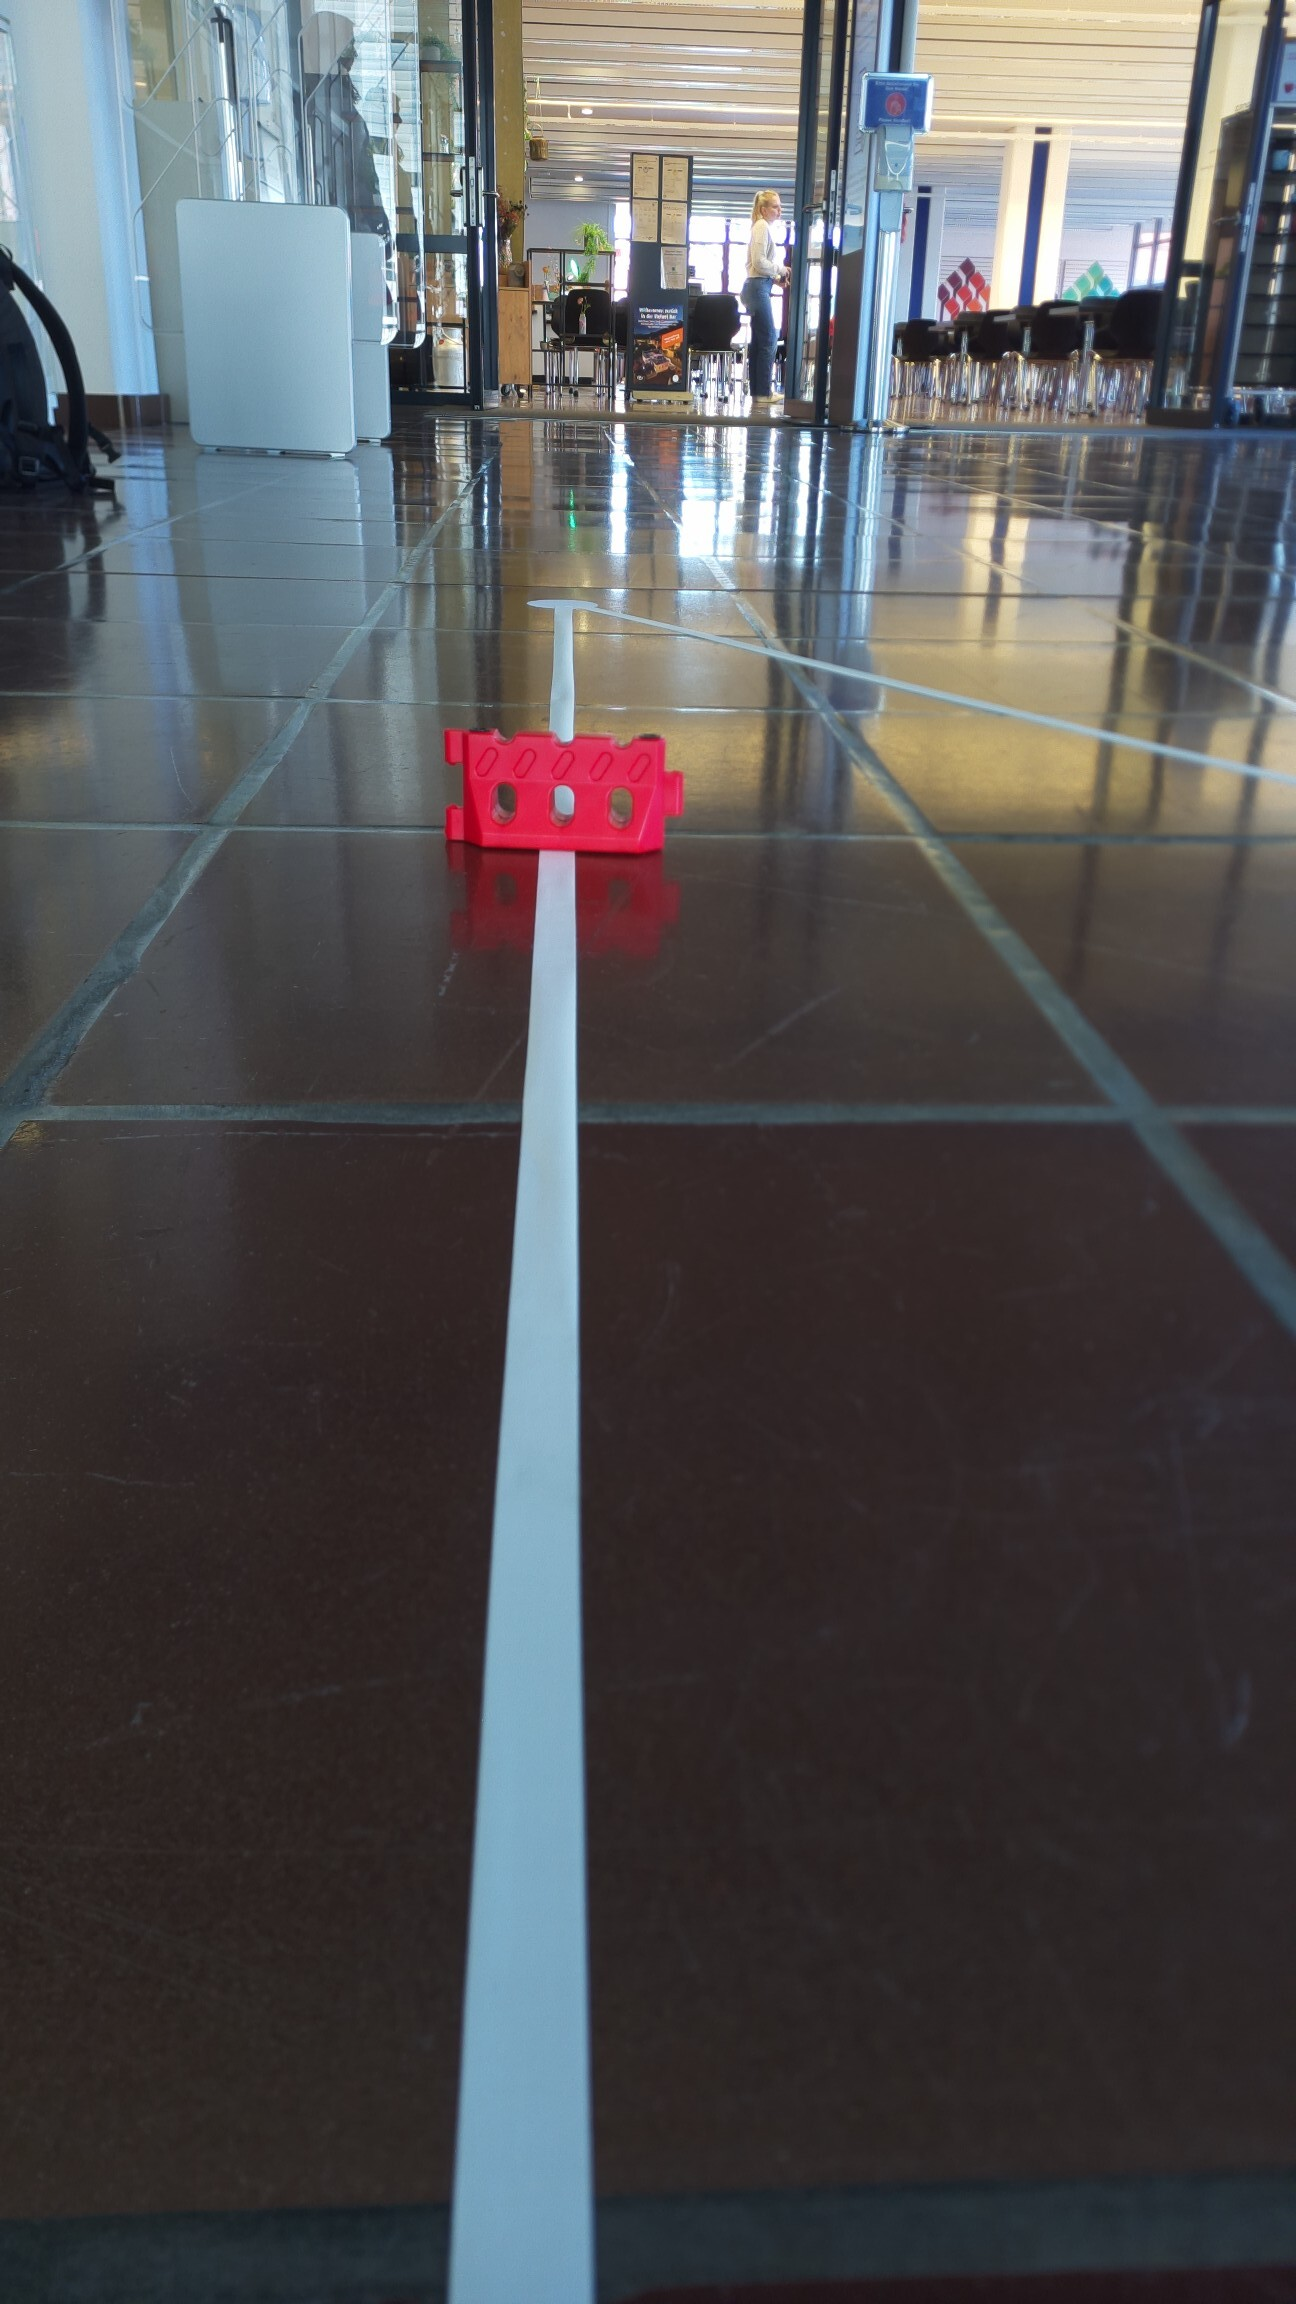
\includegraphics[width=\linewidth]{assets/IT/testing/yolo/barrier.jpg}
\end{minipage}
        &
\begin{minipage}{.18\textwidth}
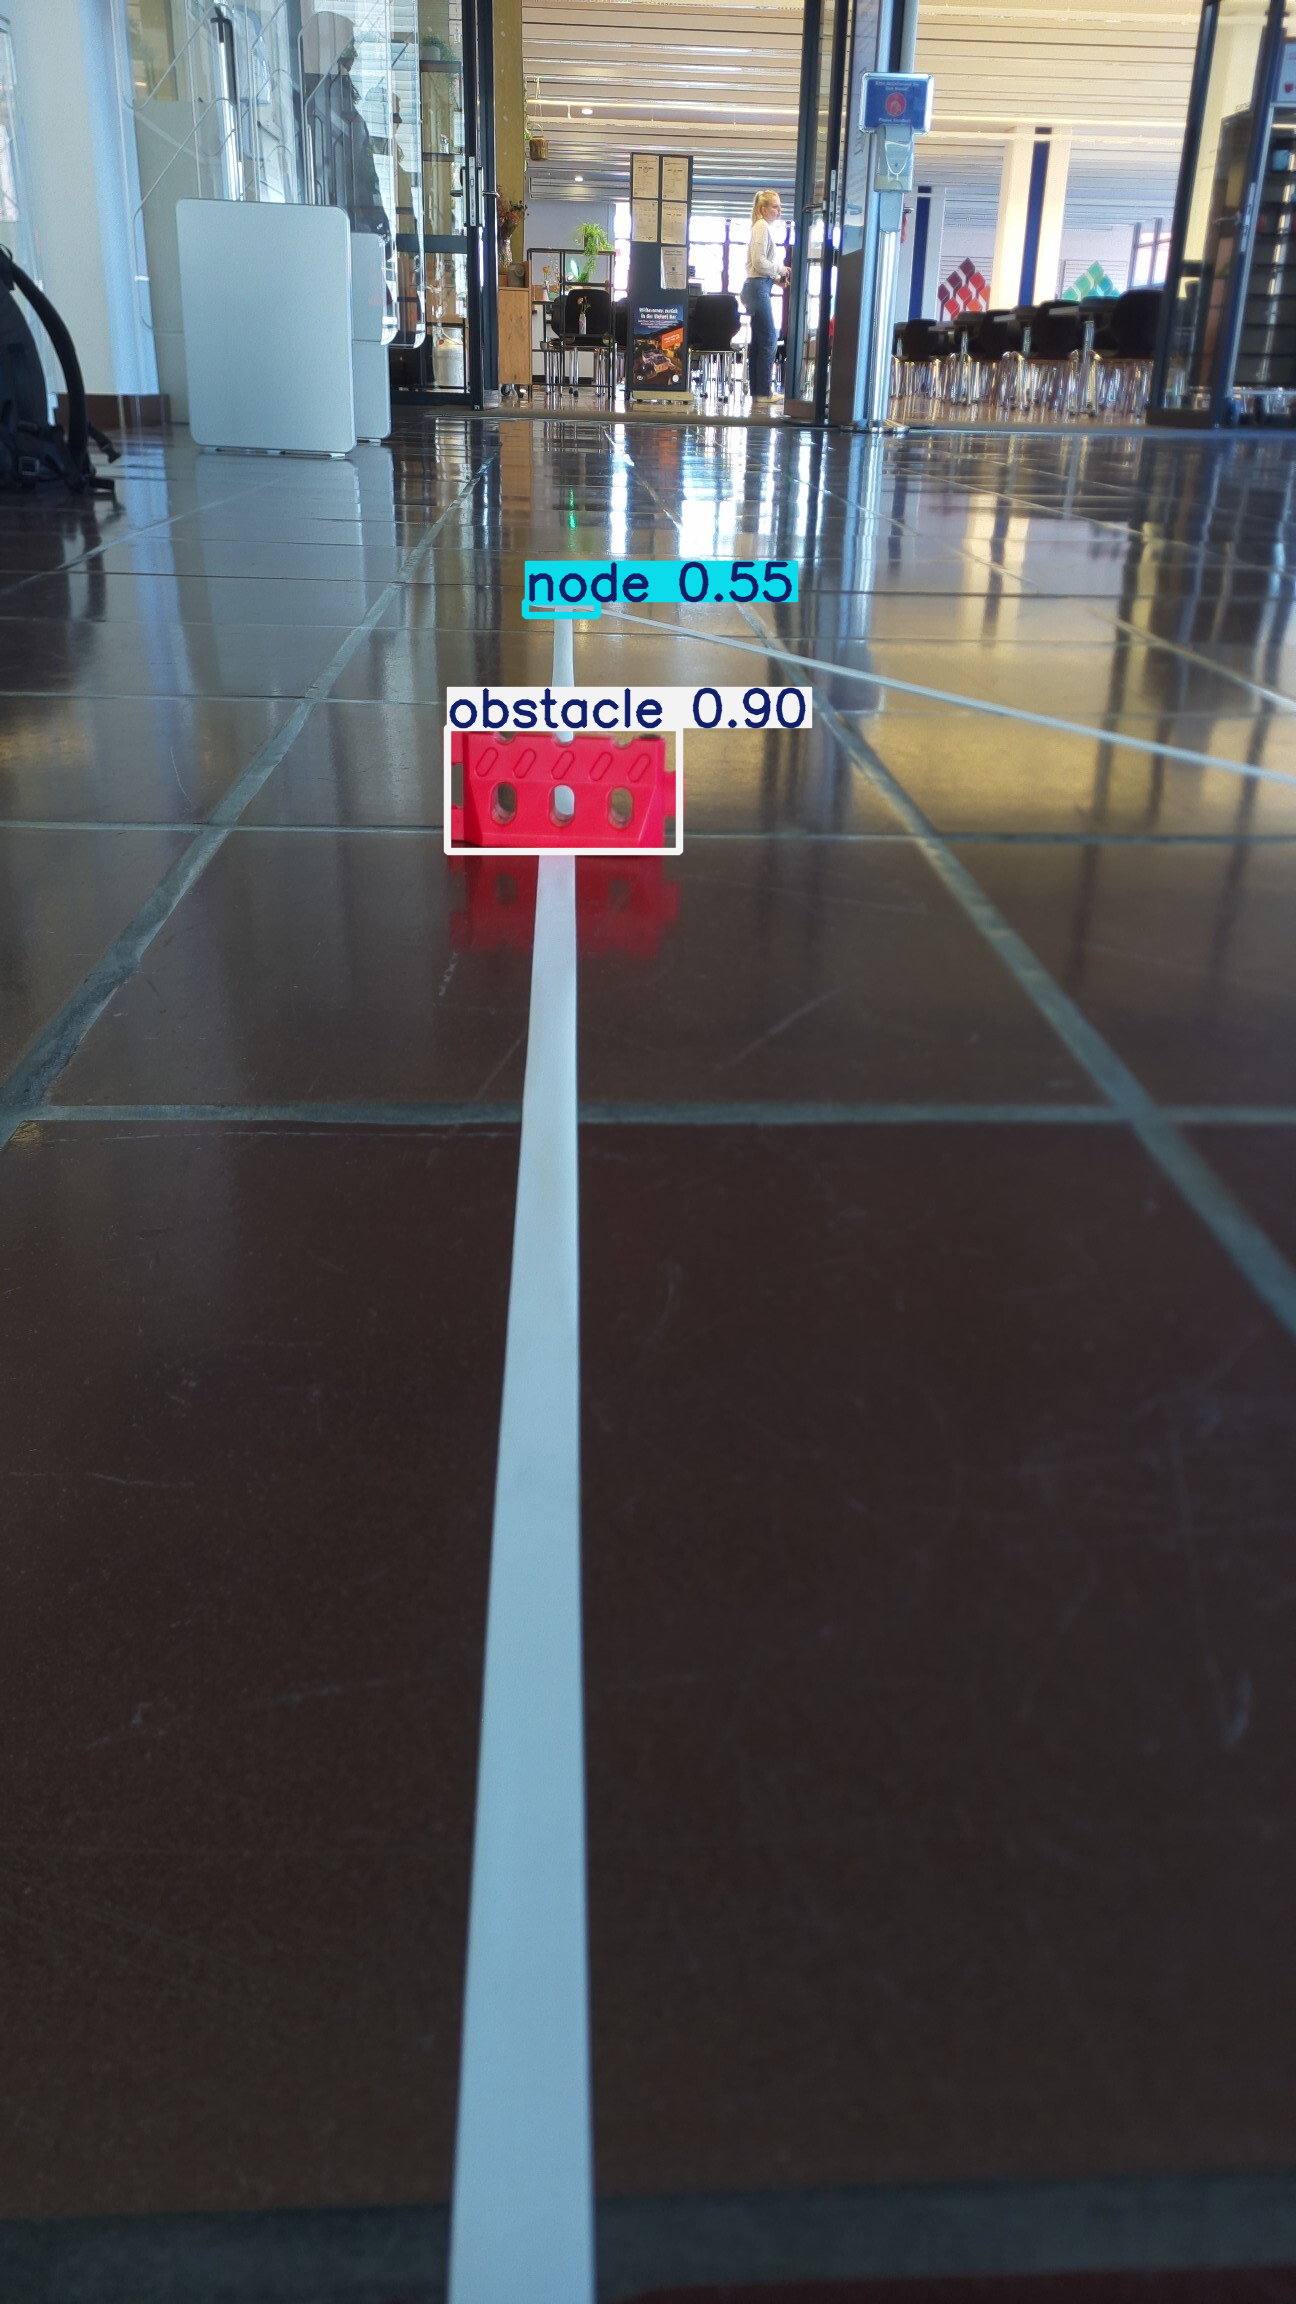
\includegraphics[width=\linewidth]{assets/IT/testing/yolo/barrier_annot.png}
\end{minipage}        
        &Barriere erkannt.&Barriere erkannt.& Erfüllt\\
        \hline
        2&
\begin{minipage}{.18\textwidth}
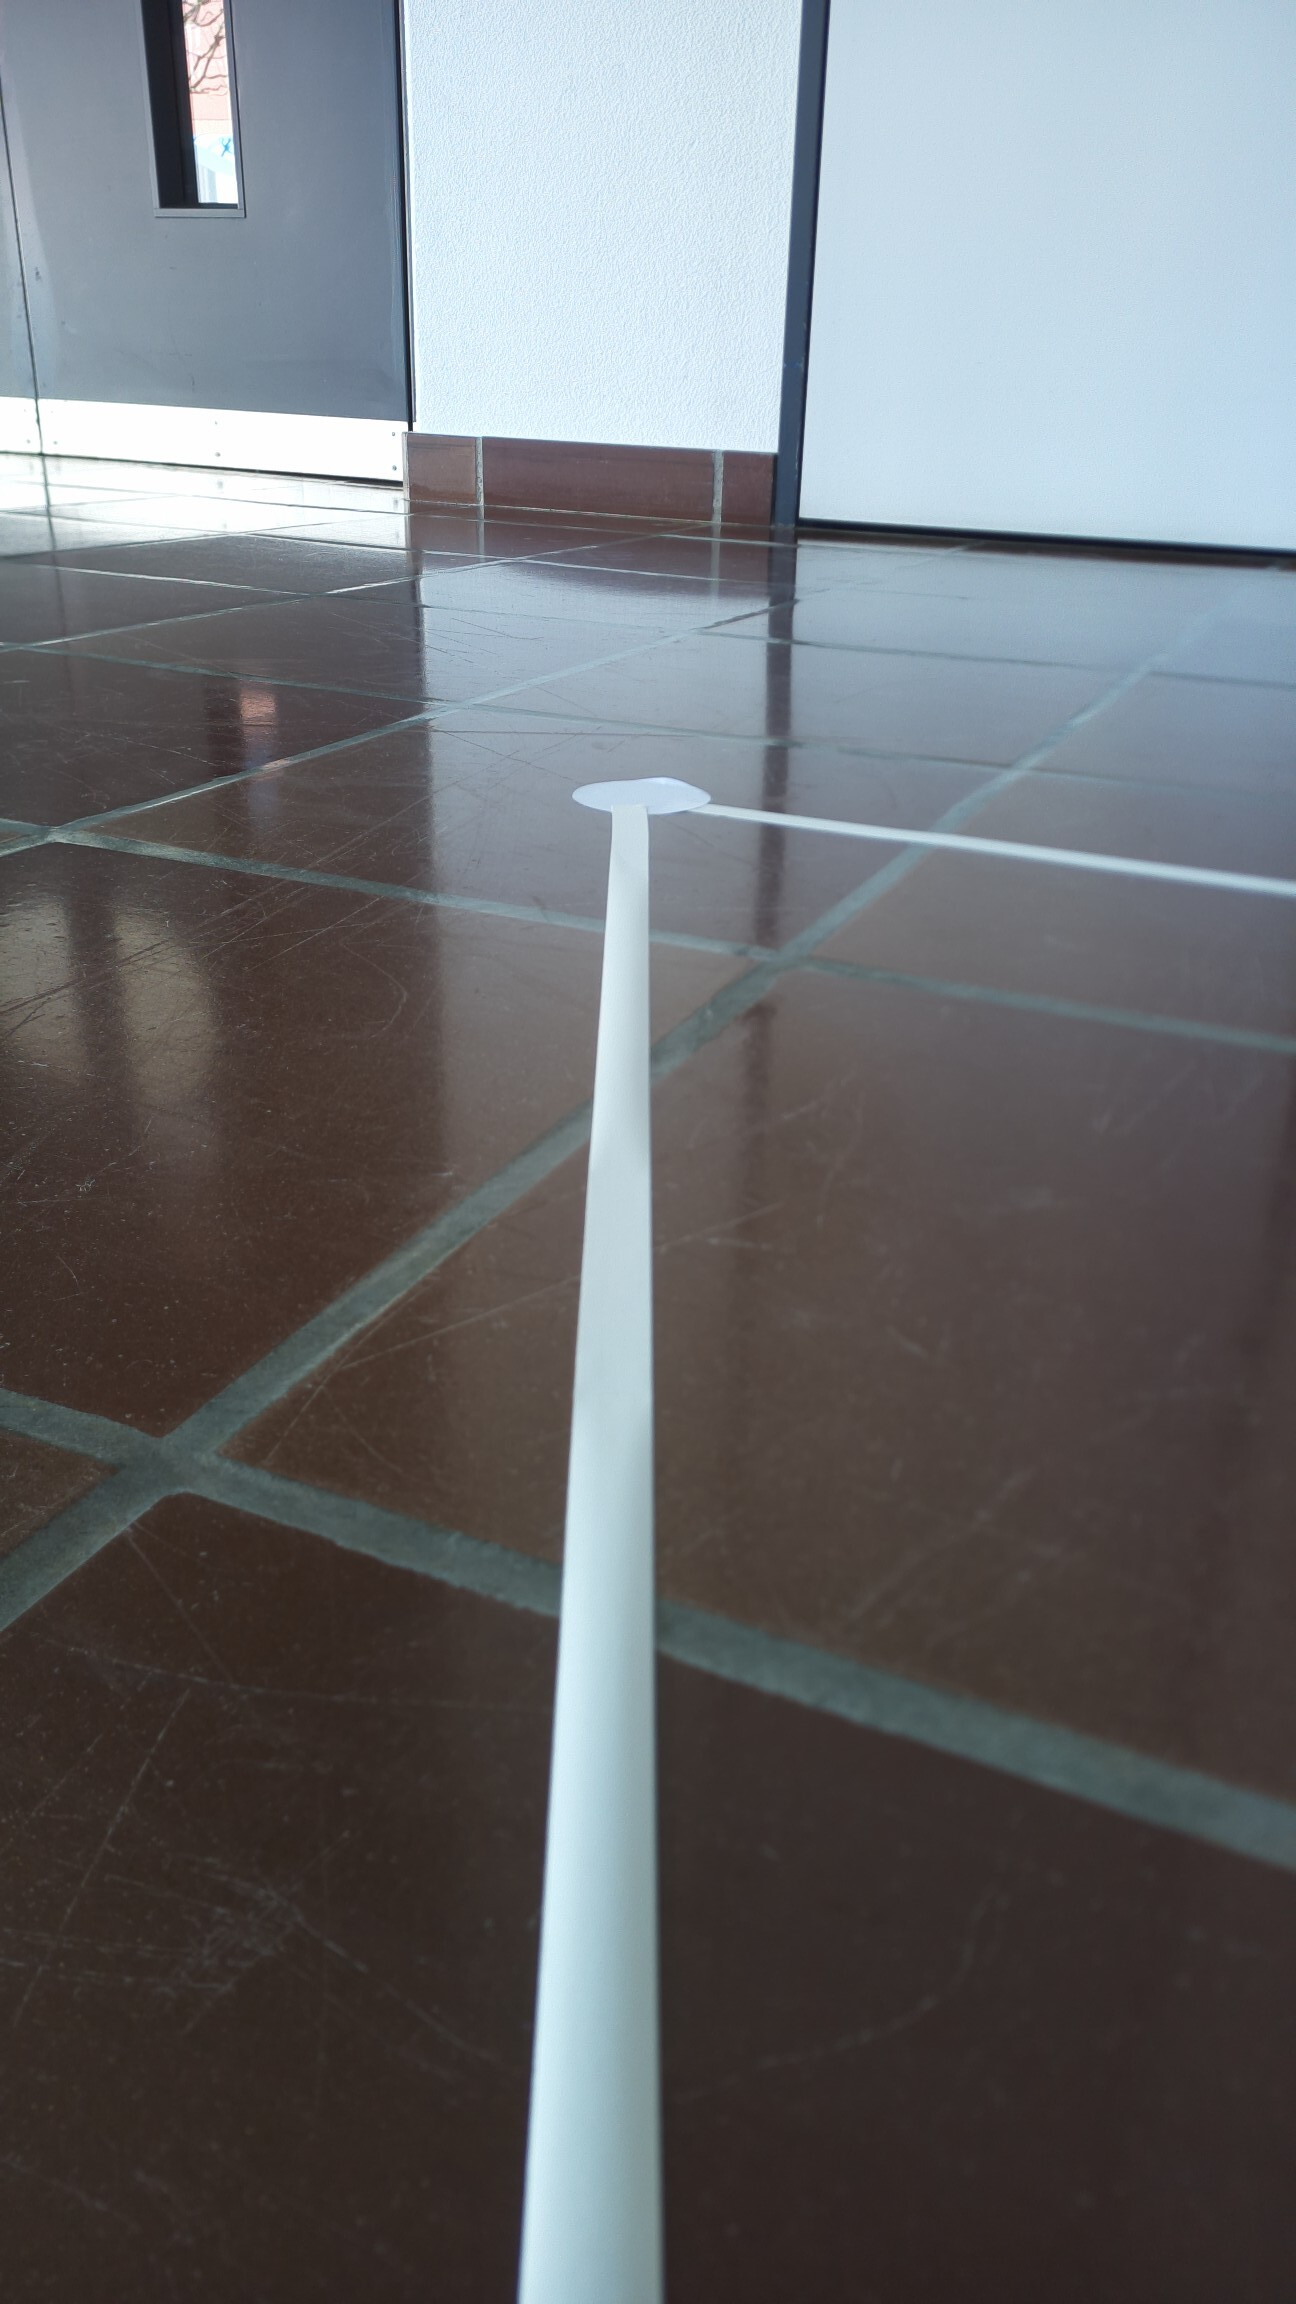
\includegraphics[width=\linewidth]{assets/IT/testing/yolo/node.jpg}
\end{minipage}
        &
\begin{minipage}{.18\textwidth}
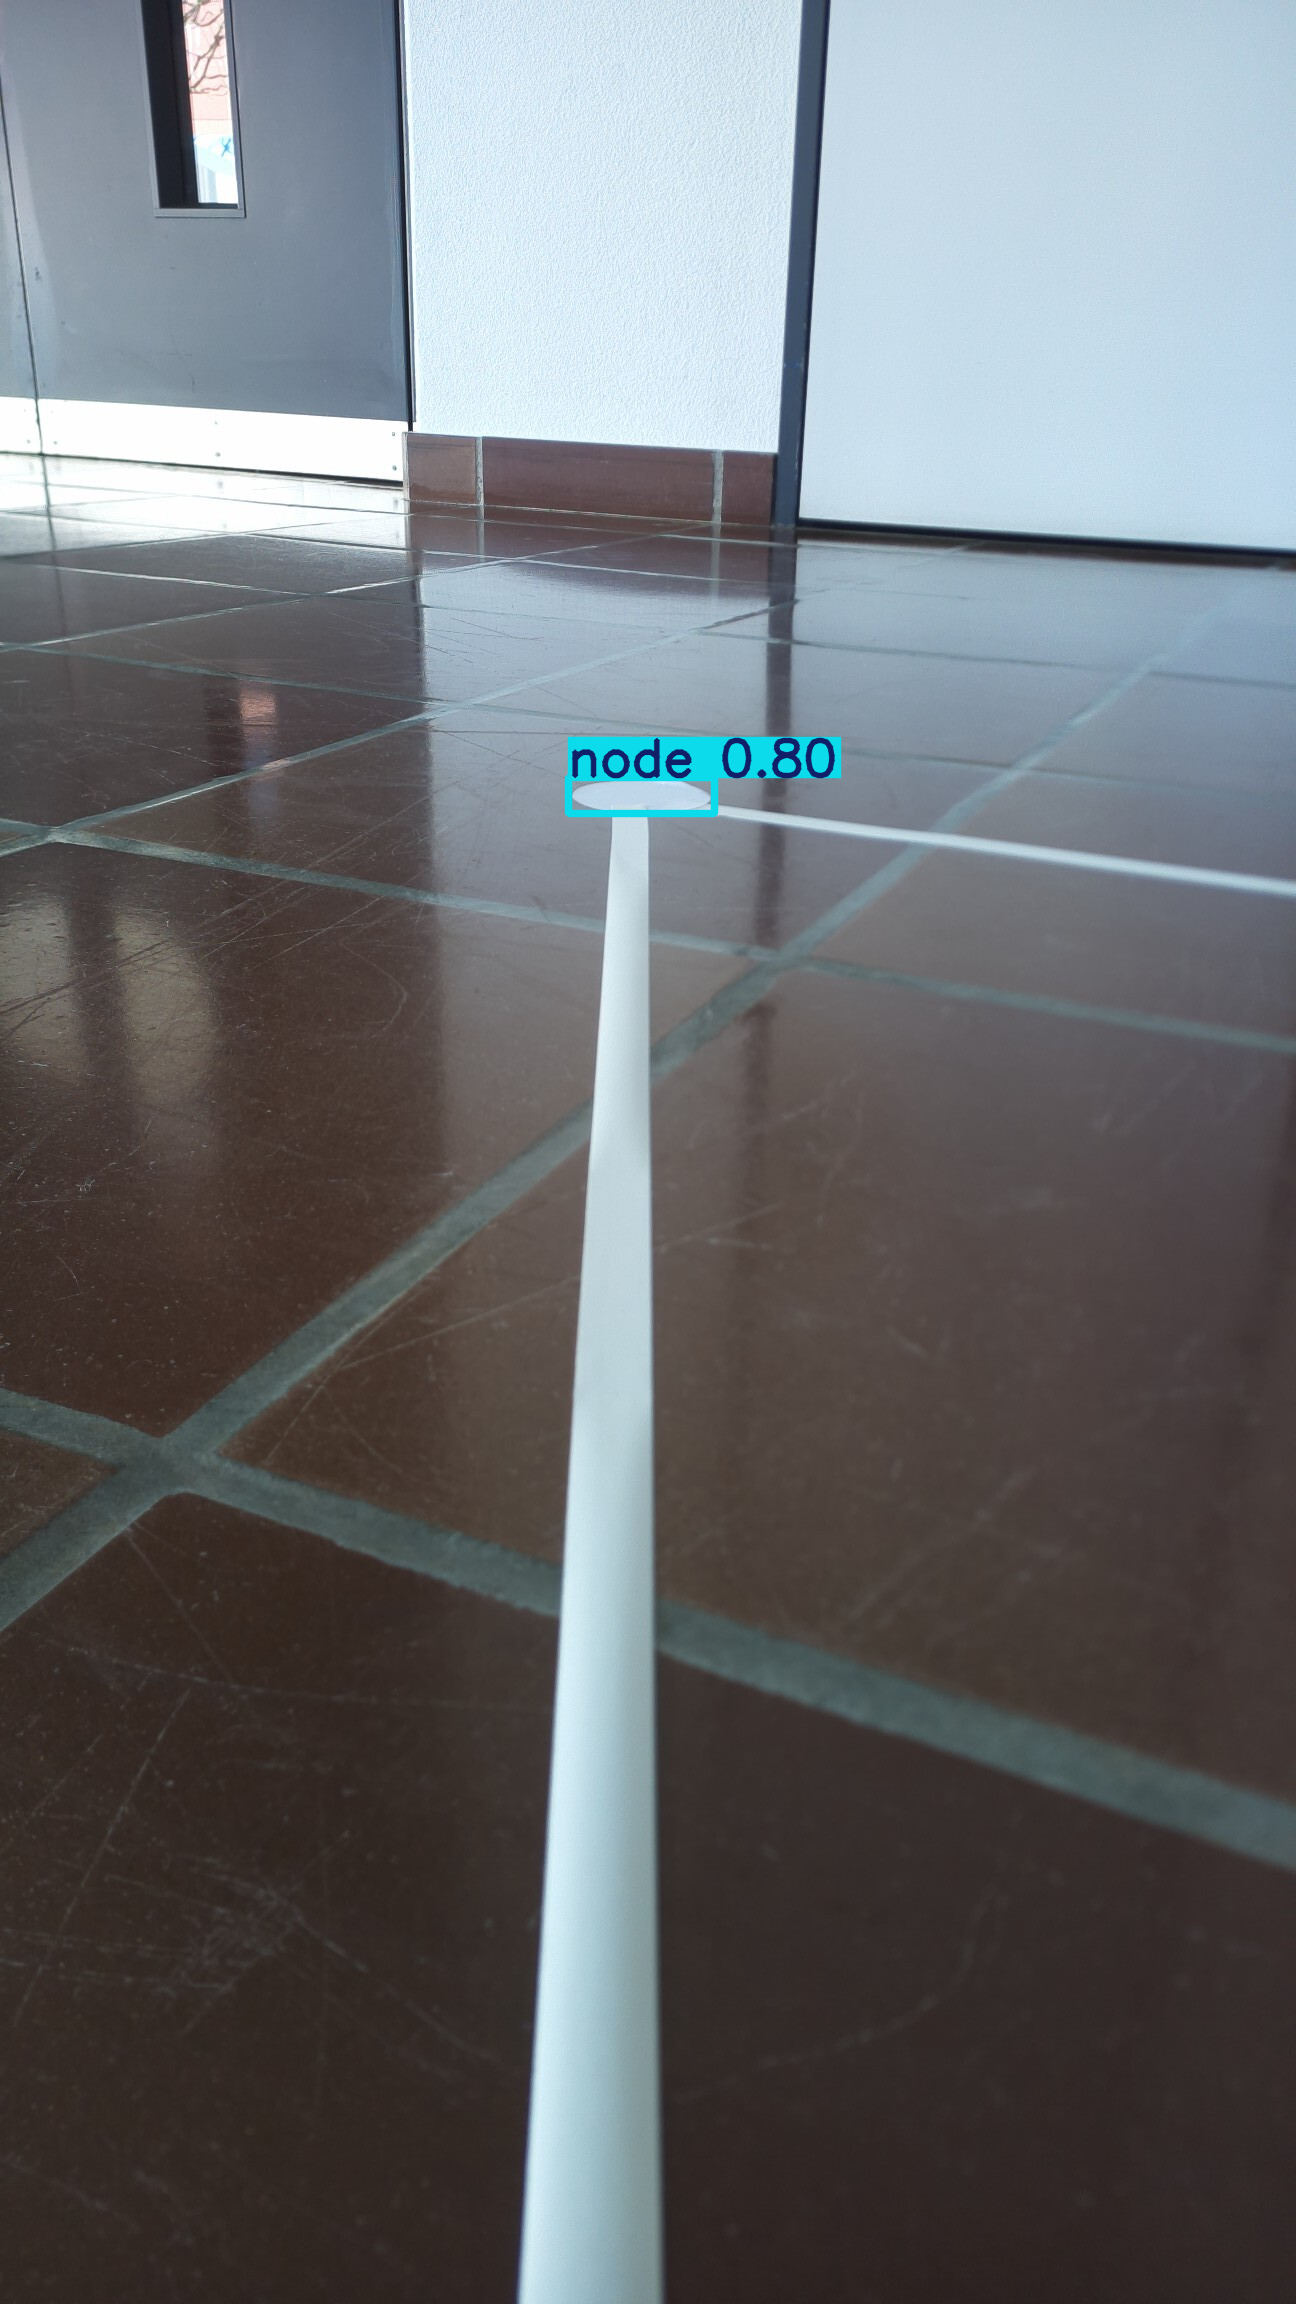
\includegraphics[width=\linewidth]{assets/IT/testing/yolo/node_annot.png}
\end{minipage}        
        &Knoten erkannt.&Knoten erkannt.& Erfüllt\\
        \hline

        3&
\begin{minipage}{.18\textwidth}
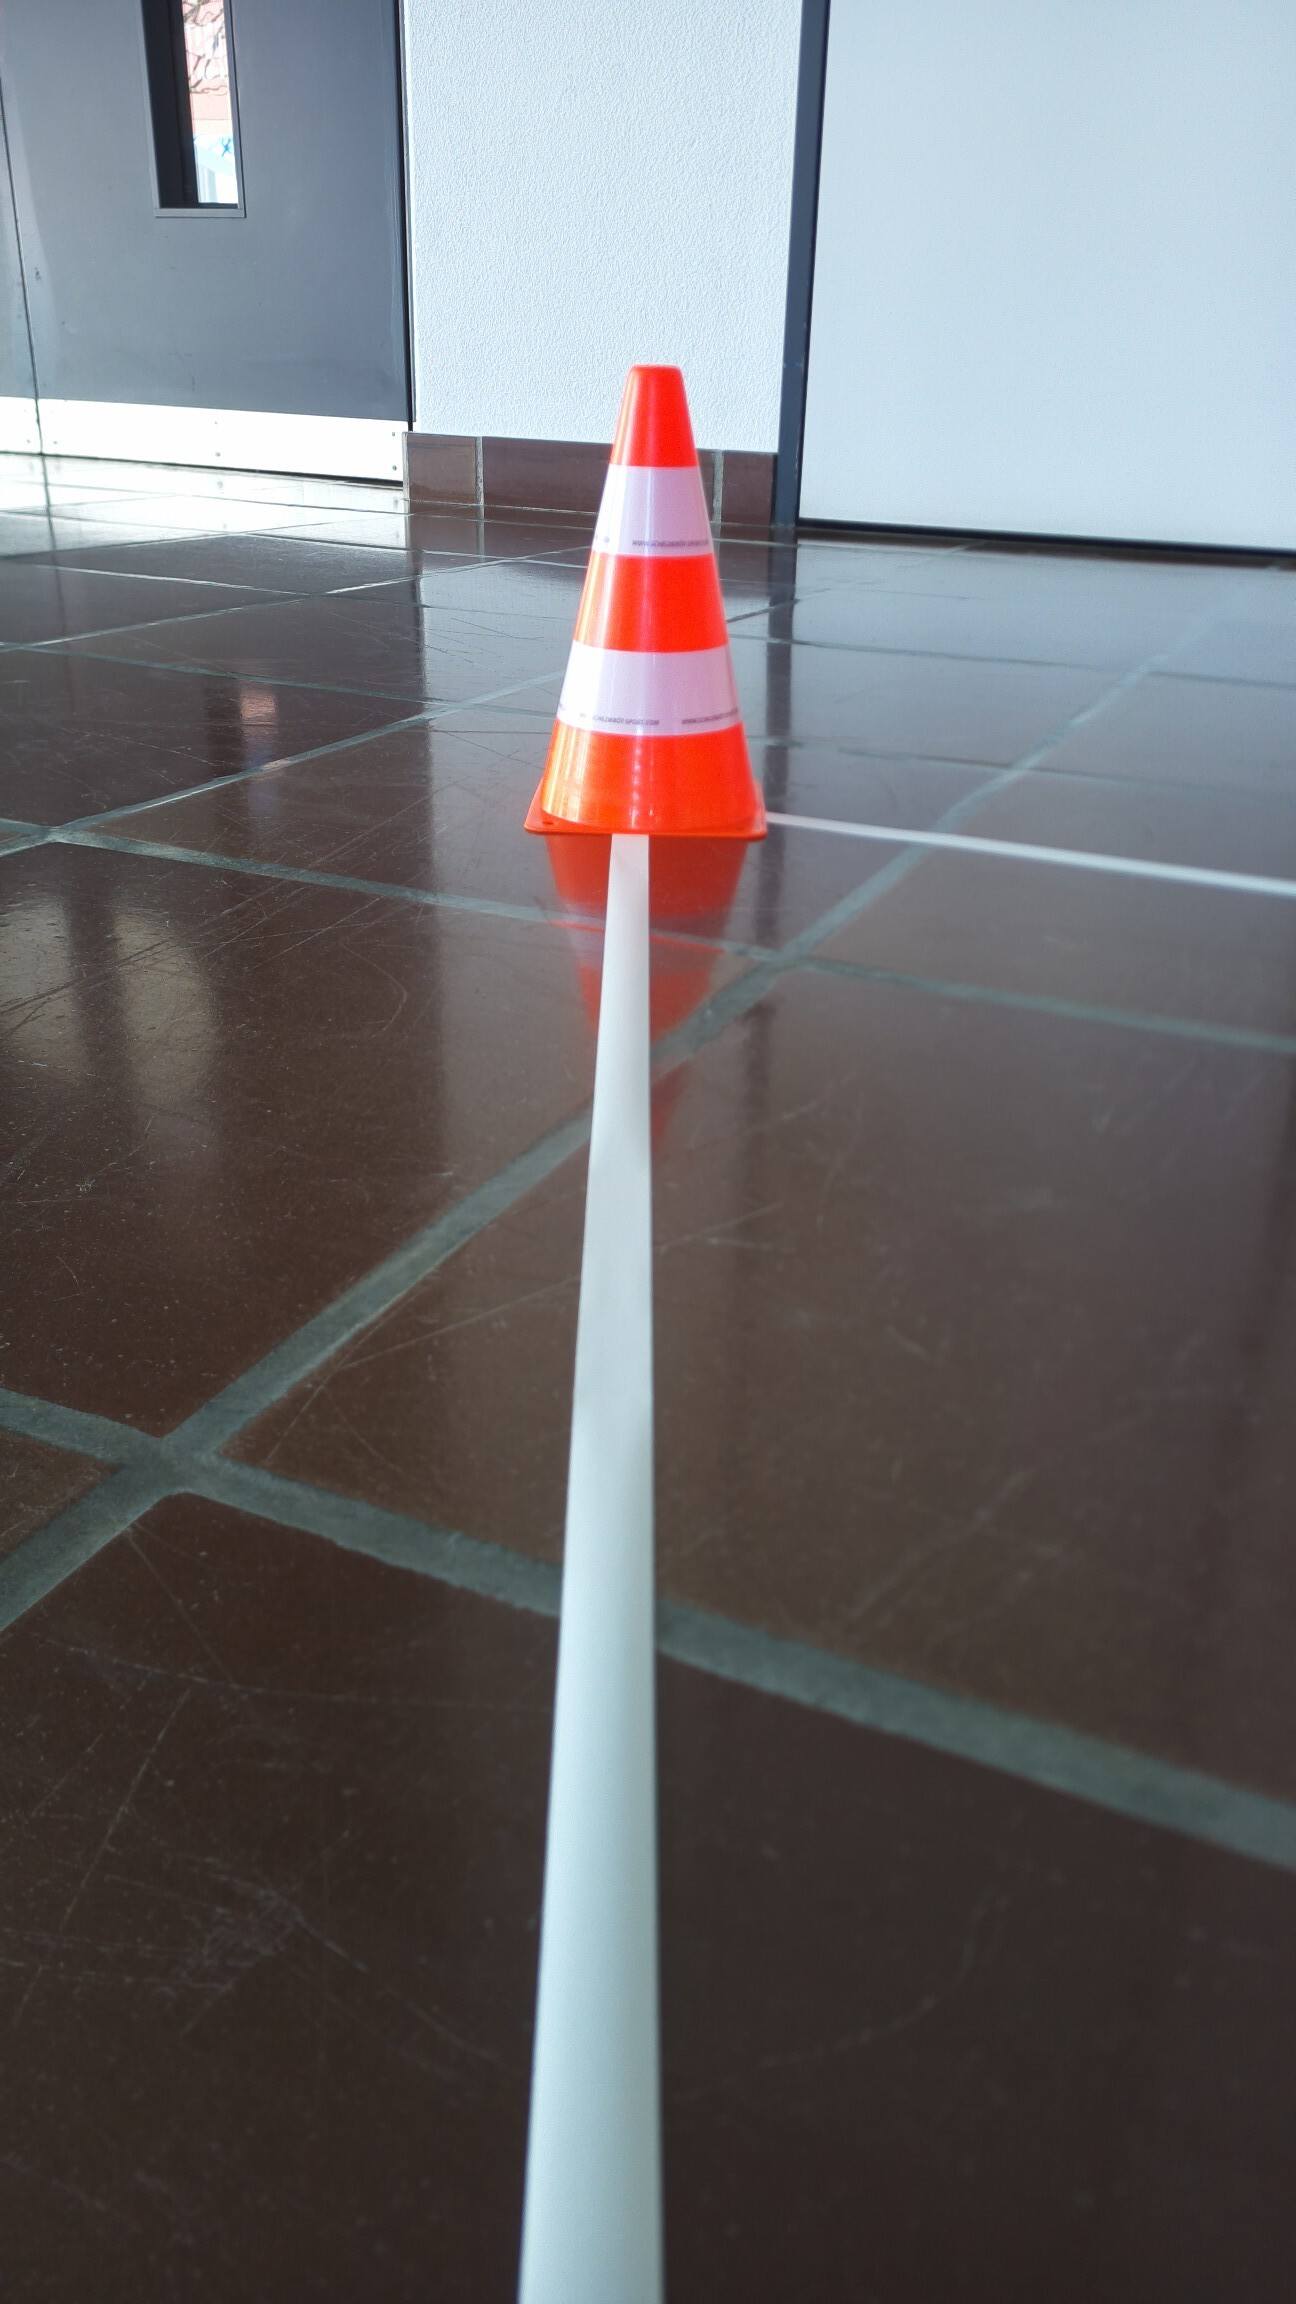
\includegraphics[width=\linewidth]{assets/IT/testing/yolo/pylon.jpg}
\end{minipage}
        &
\begin{minipage}{.18\textwidth}
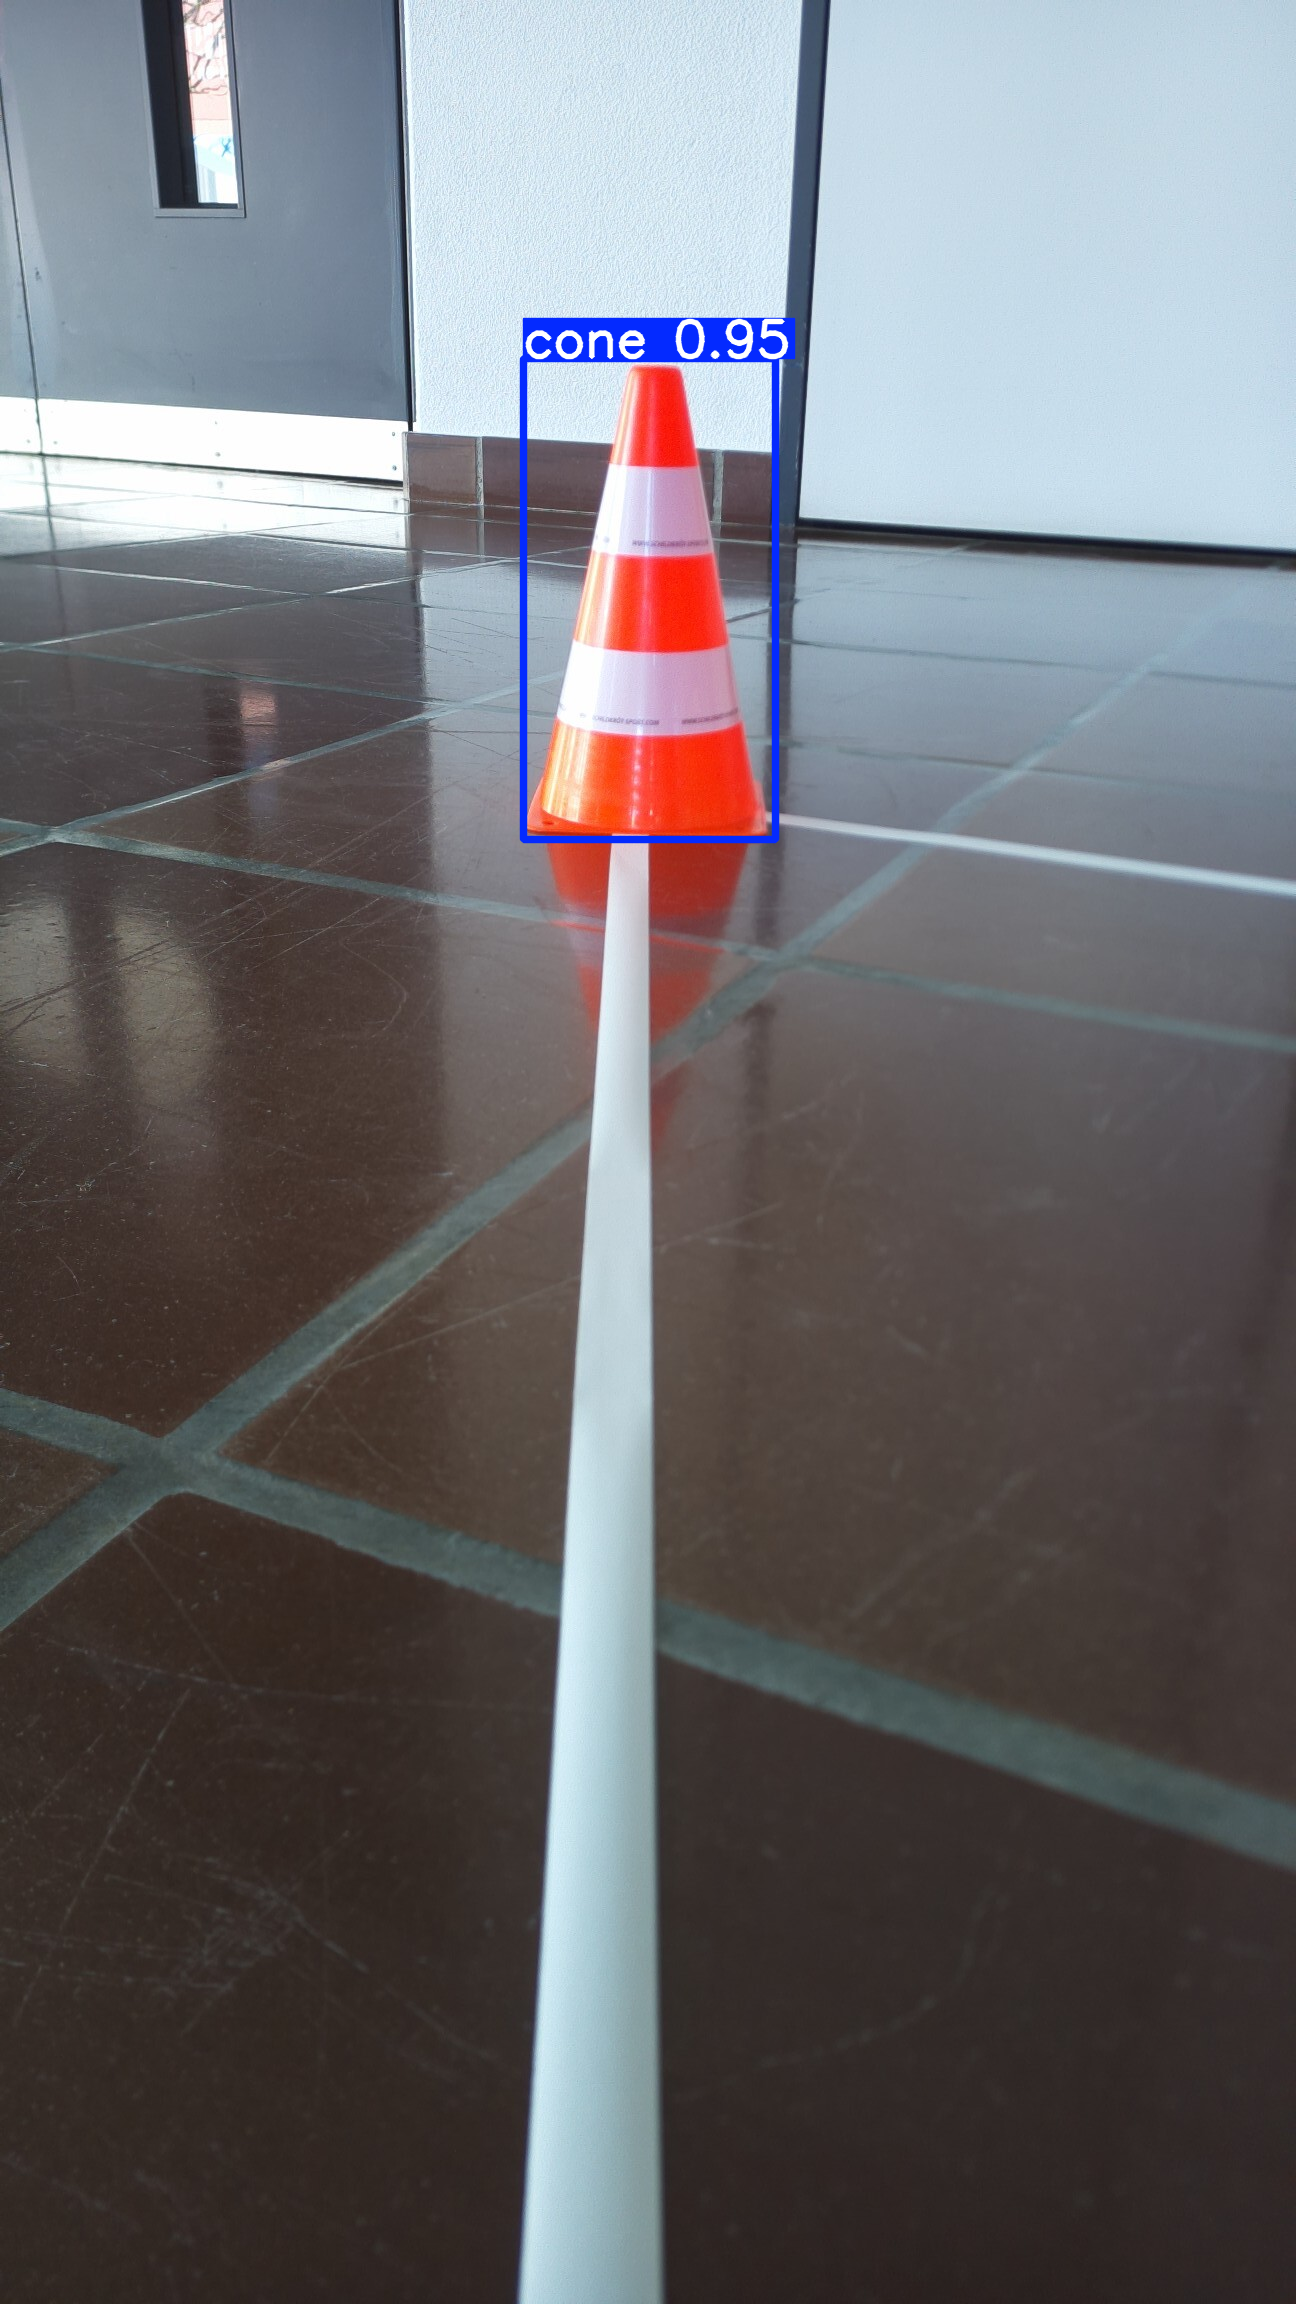
\includegraphics[width=\linewidth]{assets/IT/testing/yolo/pylon_annot.png}
\end{minipage}        
        &Pylone erkannt.&Pylone erkannt.& Erfüllt\\
        \hline


        4&
\begin{minipage}{.18\textwidth}
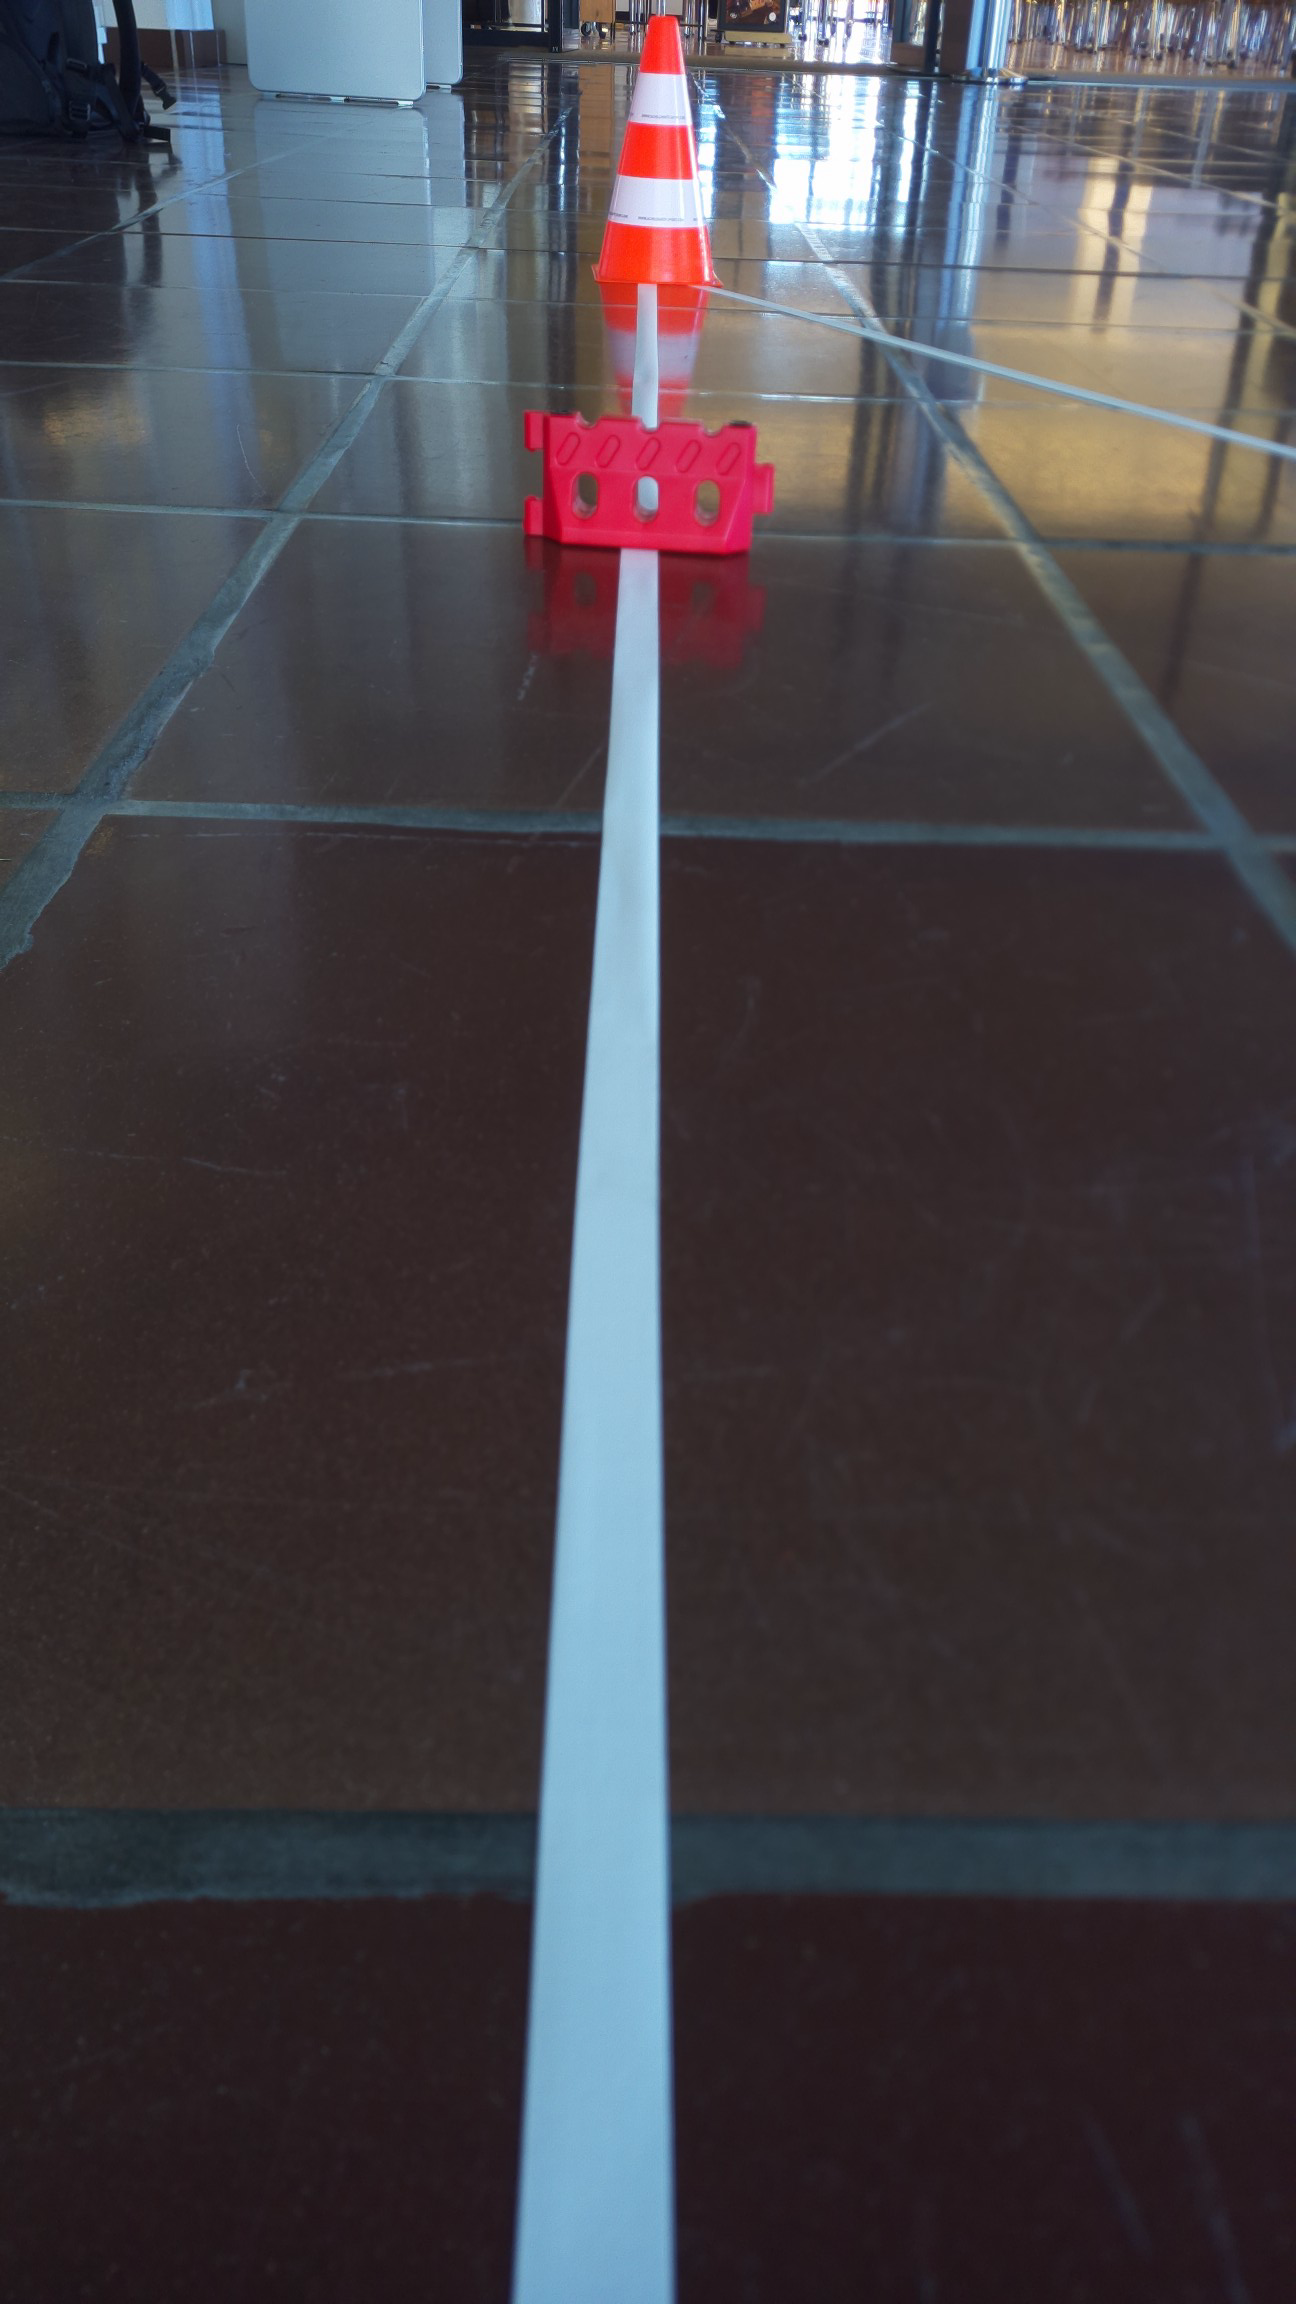
\includegraphics[width=\linewidth]{assets/IT/testing/yolo/pylon_behind_obst.png}
\end{minipage}
        &
\begin{minipage}{.18\textwidth}
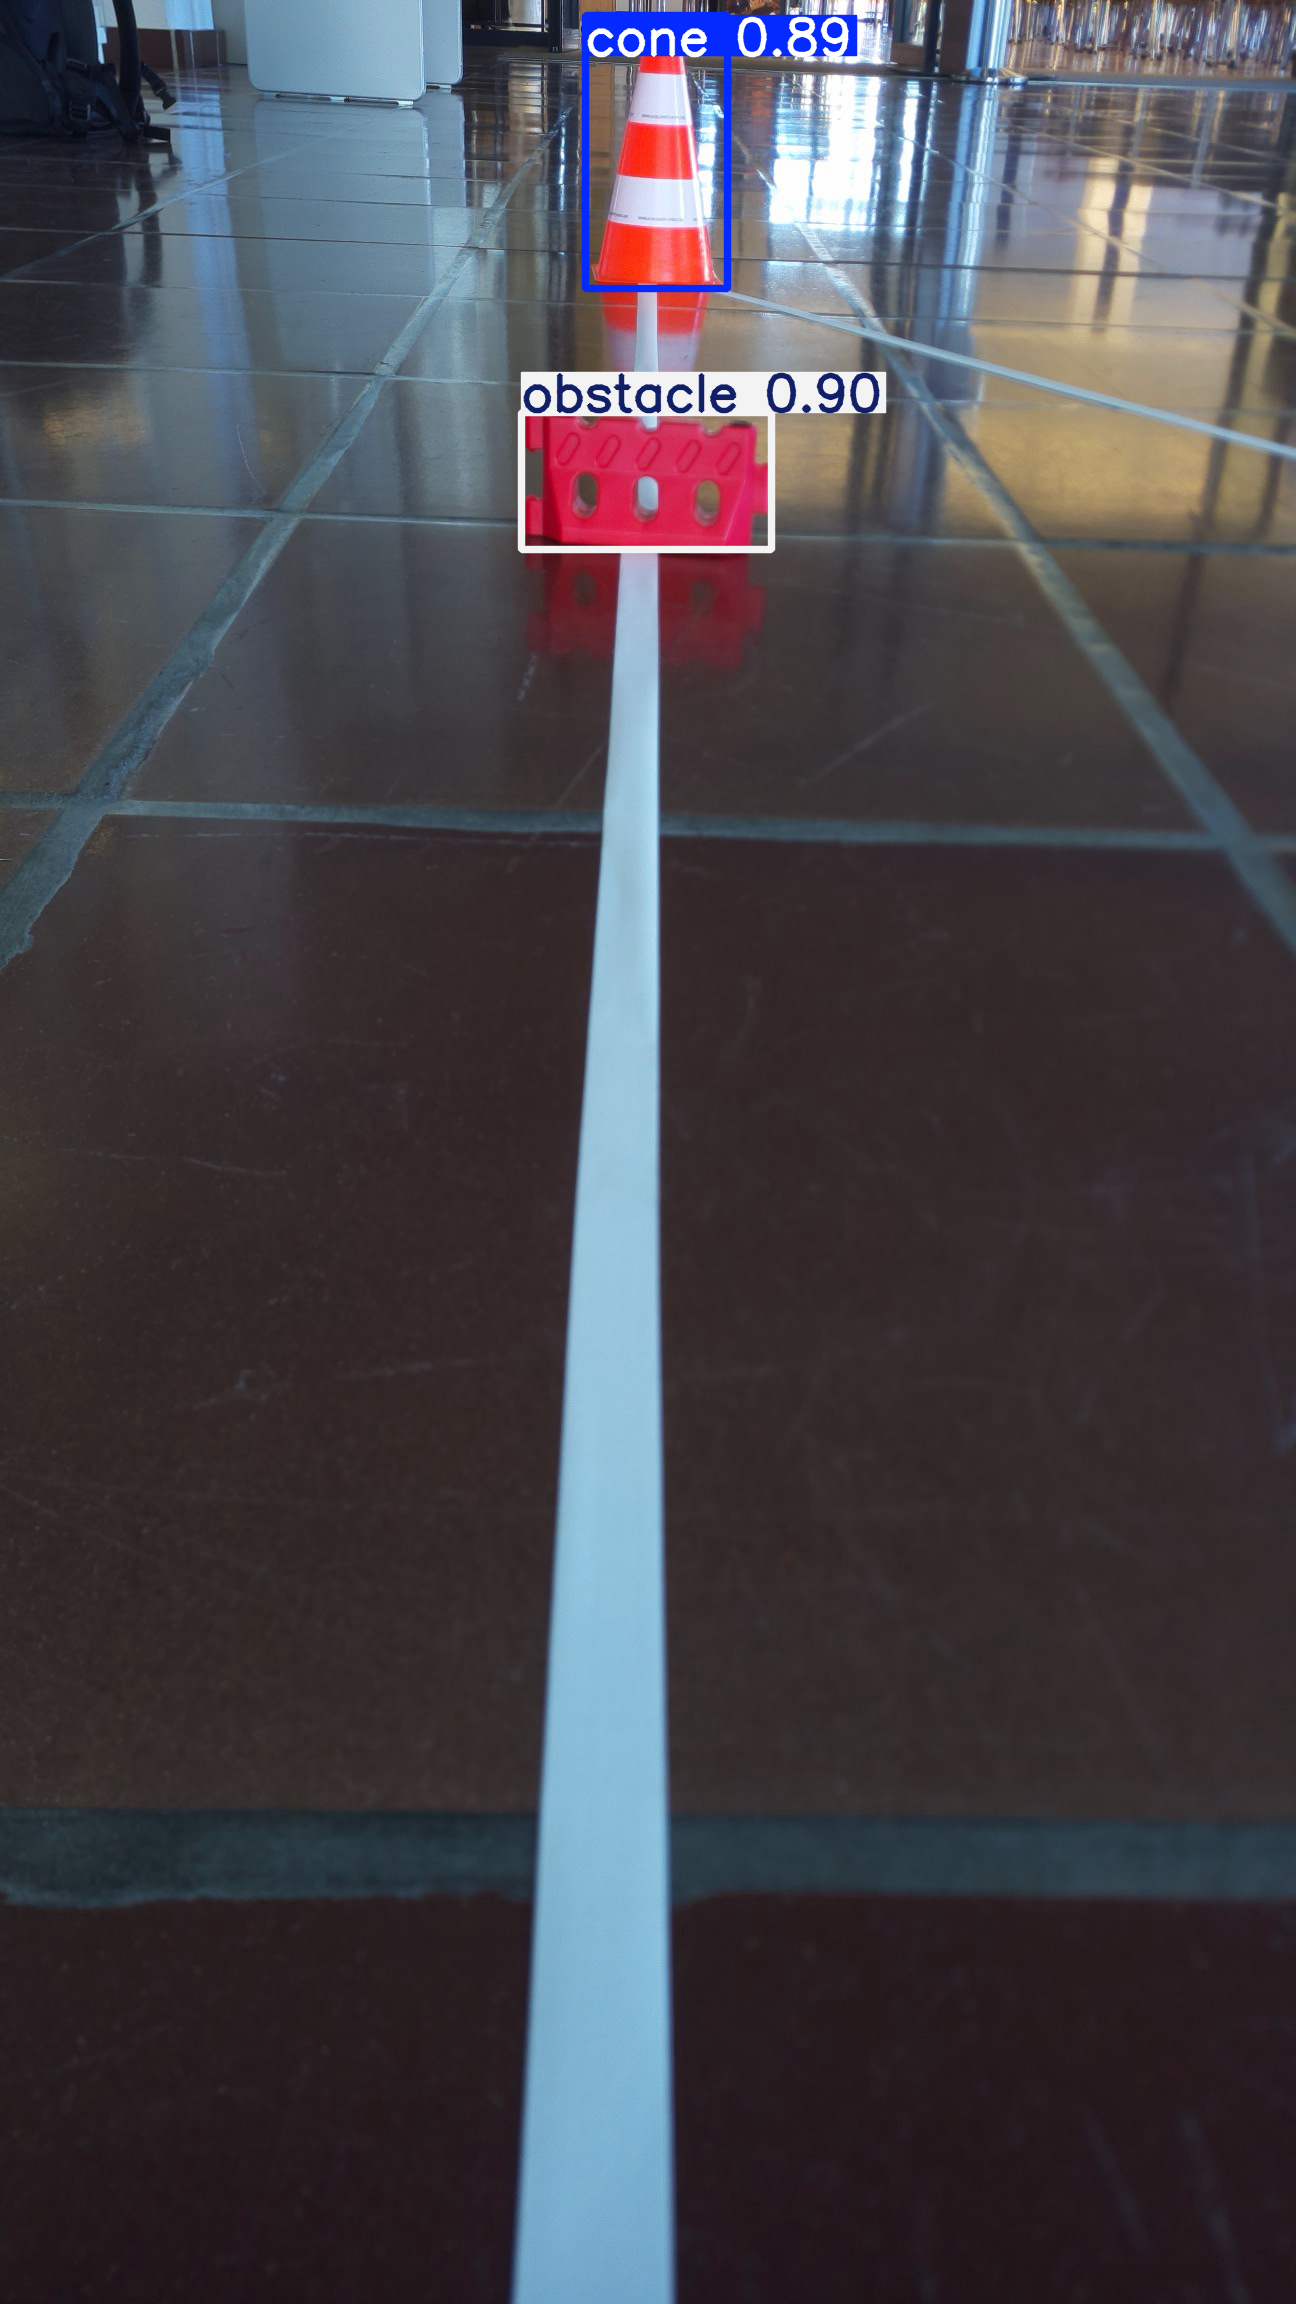
\includegraphics[width=\linewidth]{assets/IT/testing/yolo/pylon_behind_obst_annot.png}
\end{minipage}        
        &Pylone erkannt.&Pylone erkannt.& Erfüllt\\
        \hline

         \end{tabularx}
\end{table}

\newpage

\begin{table}[H]
\centering
\small
\begin{tabularx}\textwidth{|c | X |X | X | X | c | }
\hline
  \textbf{Nr} & \textbf{Bild} & \textbf{Annotiertes Bild} &\textbf{Soll} & \textbf{Ist} & \textbf{Resultat} \\
  \hline
        5&
\begin{minipage}{.18\textwidth}
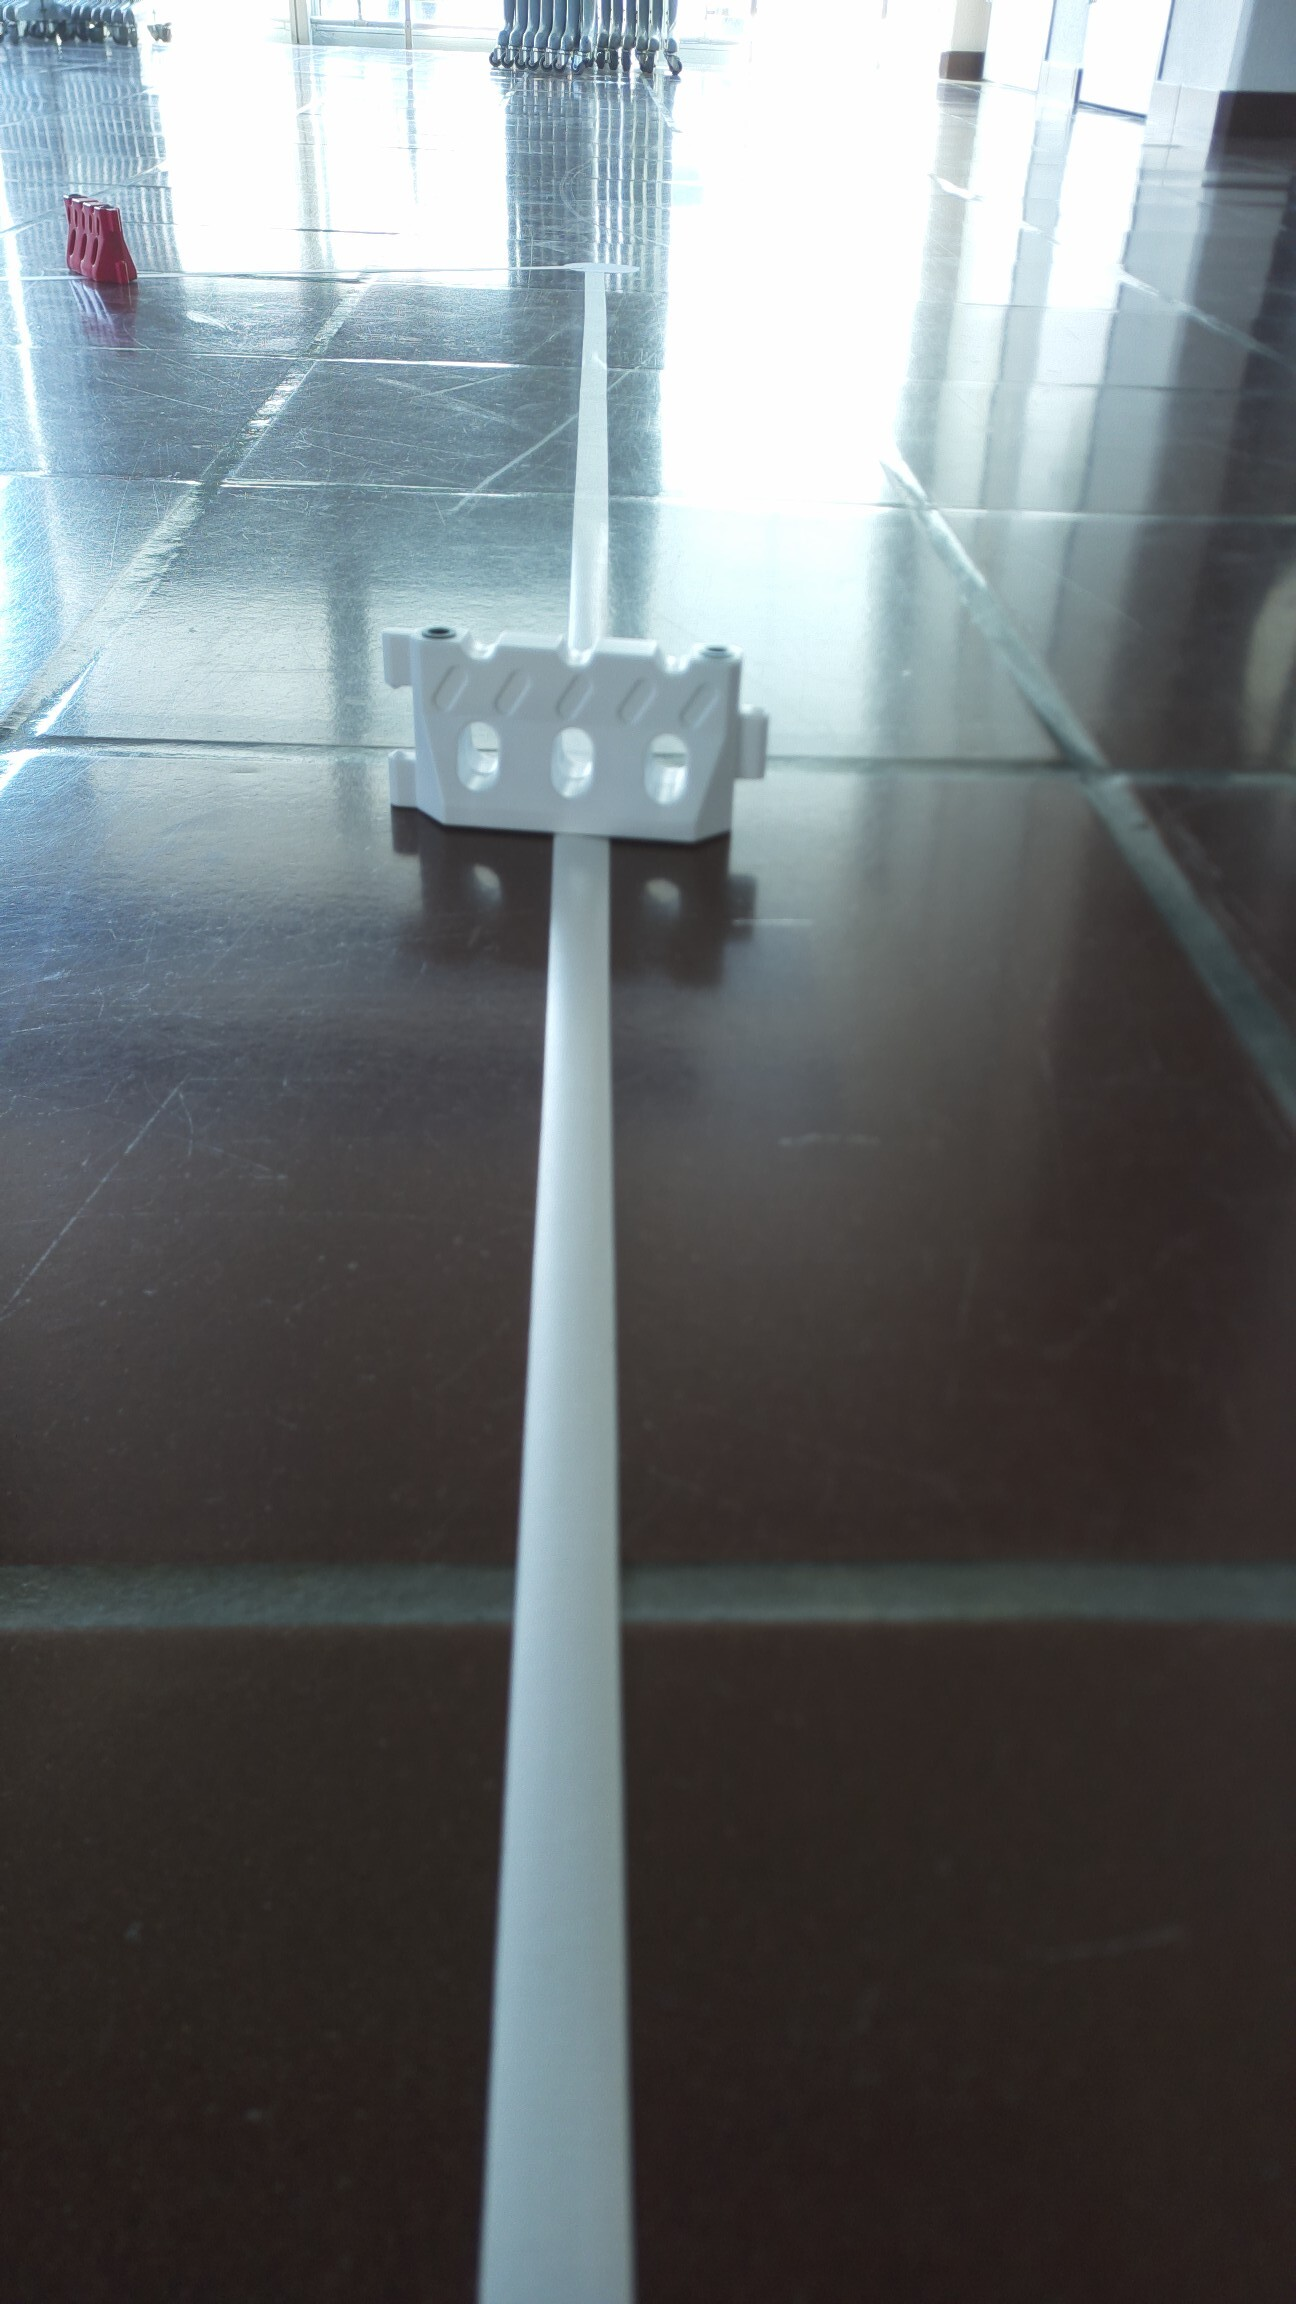
\includegraphics[width=\linewidth]{assets/IT/testing/yolo/2_barriers_1_node.jpg}
\end{minipage}
        &
\begin{minipage}{.18\textwidth}
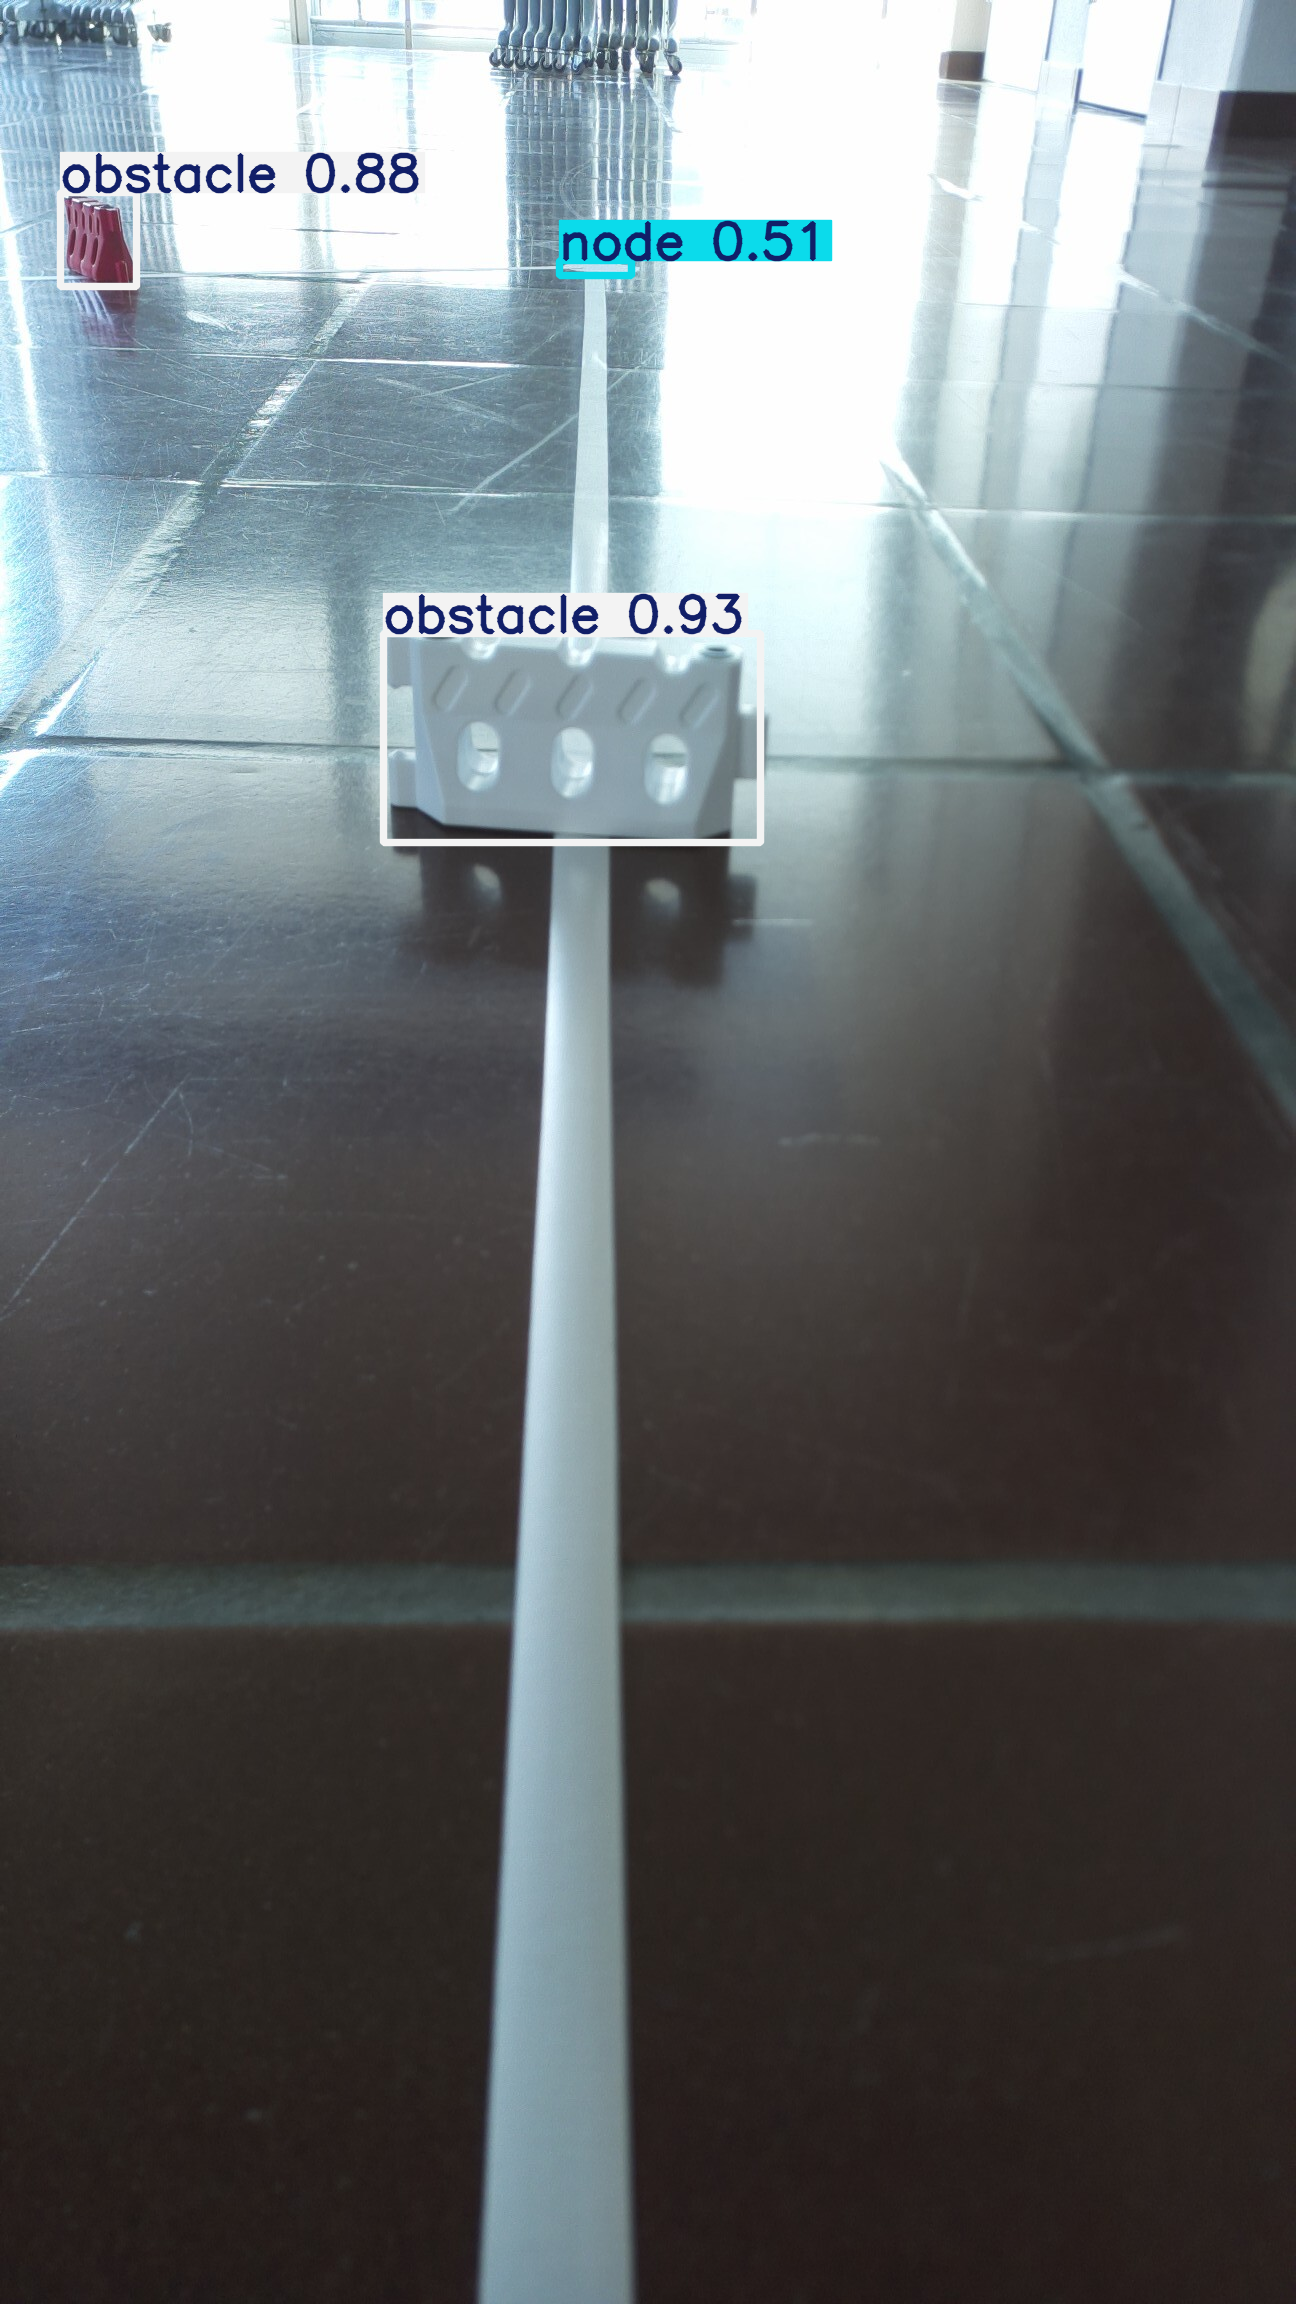
\includegraphics[width=\linewidth]{assets/IT/testing/yolo/2_barriers_1_node_annot.png}
\end{minipage}        
        &Barriere erkannt.&Barriere erkannt.&Erfüllt \\
        \hline
        6&
\begin{minipage}{.18\textwidth}
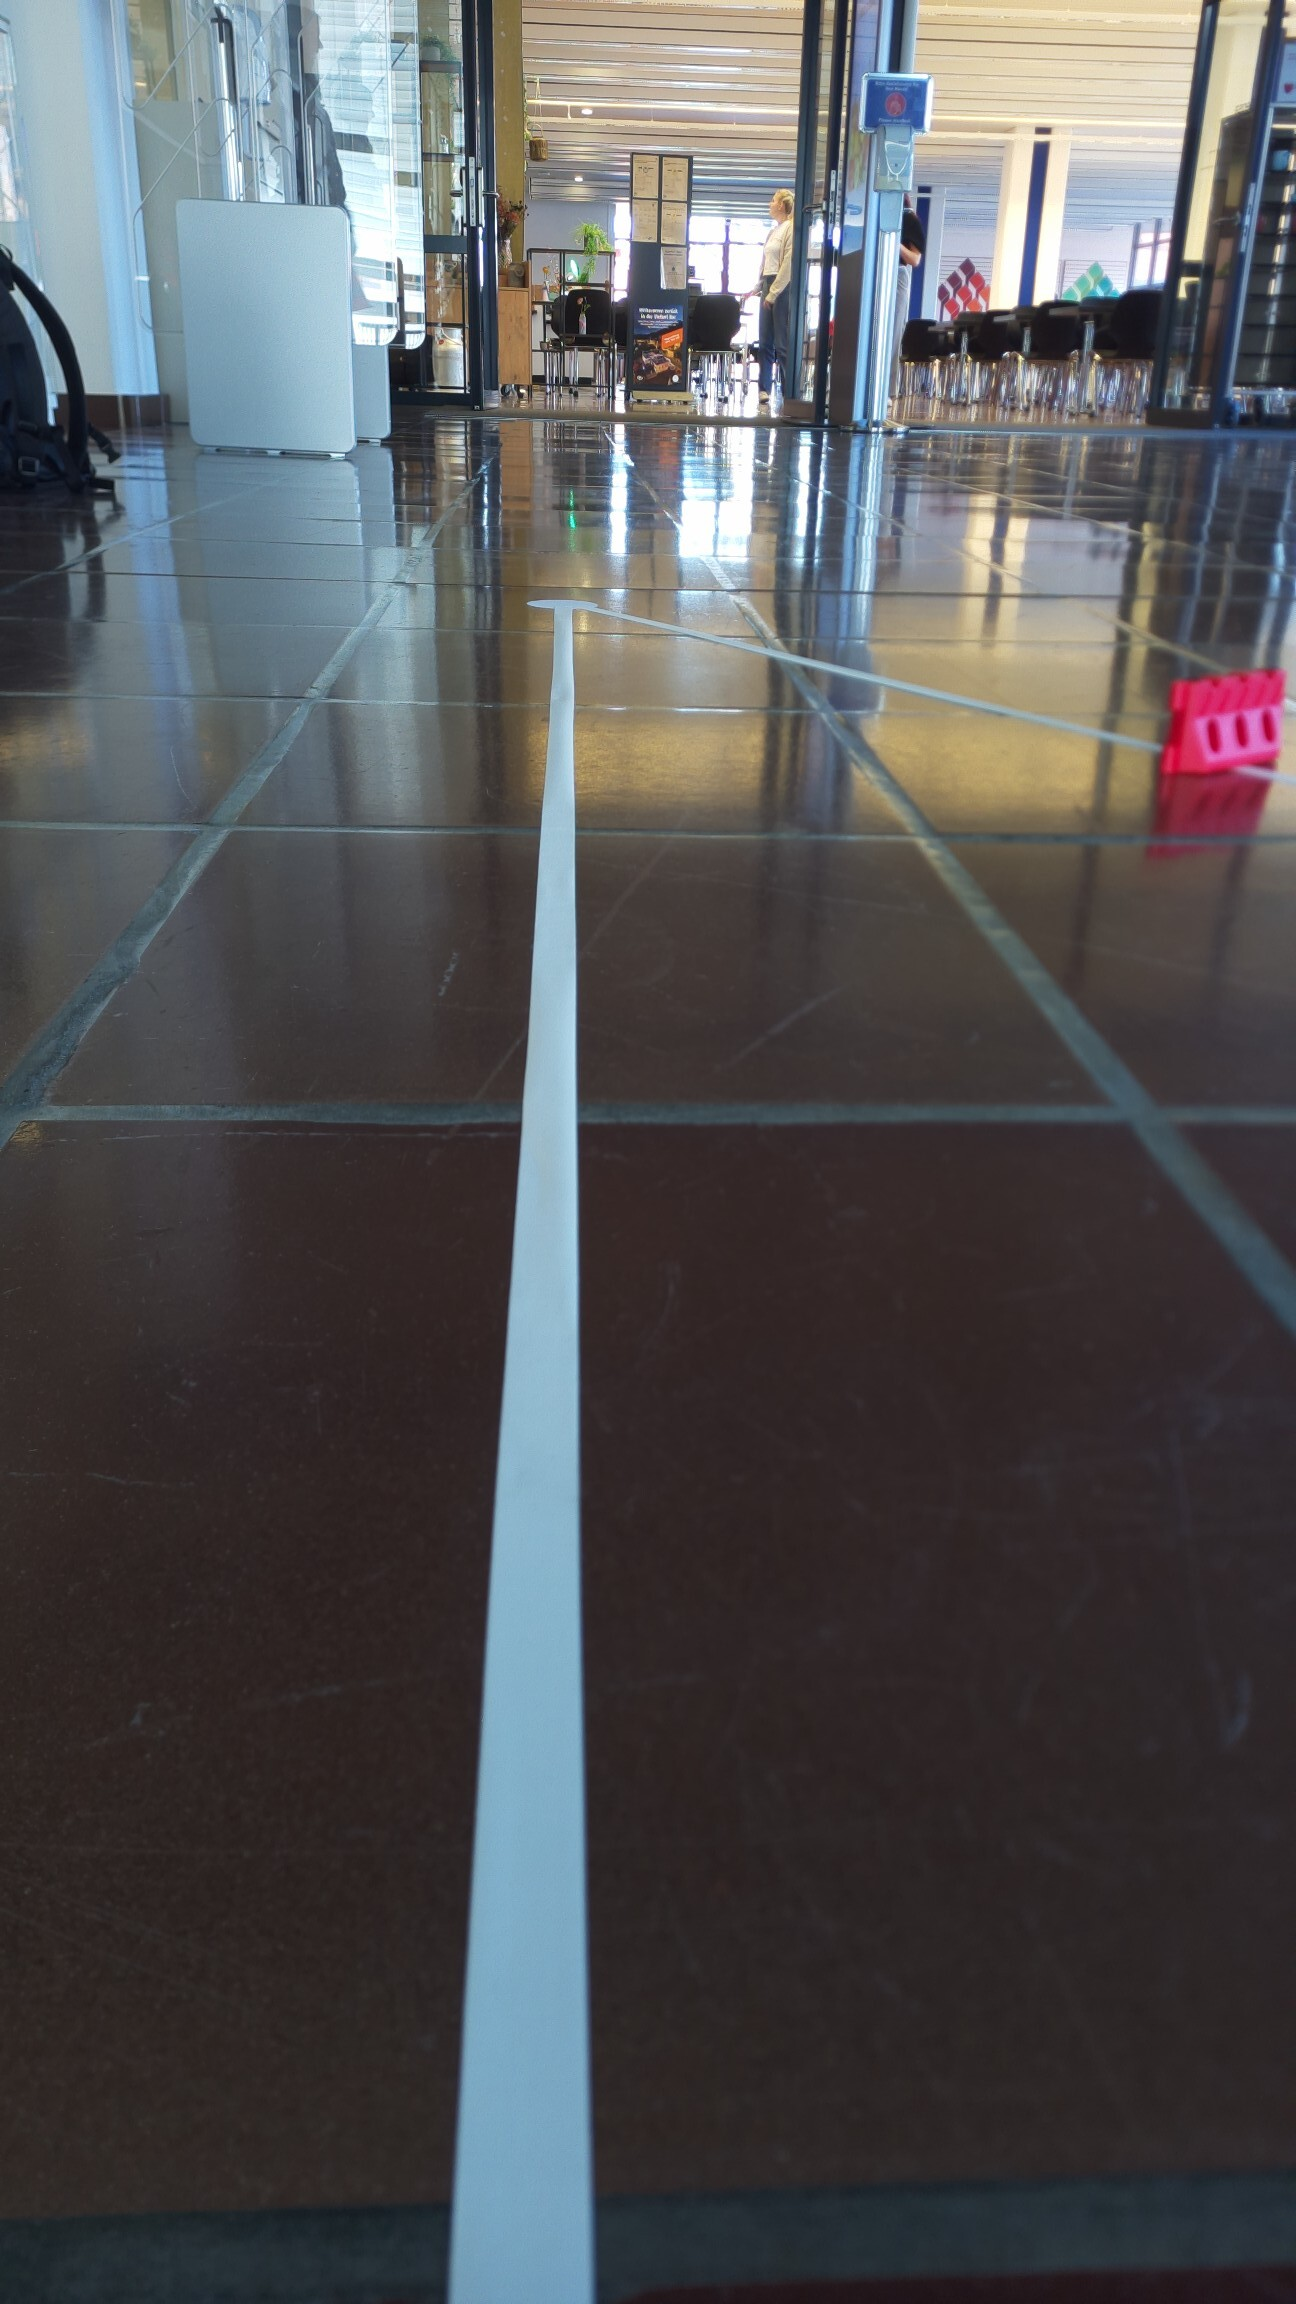
\includegraphics[width=\linewidth]{assets/IT/testing/yolo/node-obst-on-the-side.jpg}
\end{minipage}
        &
\begin{minipage}{.18\textwidth}
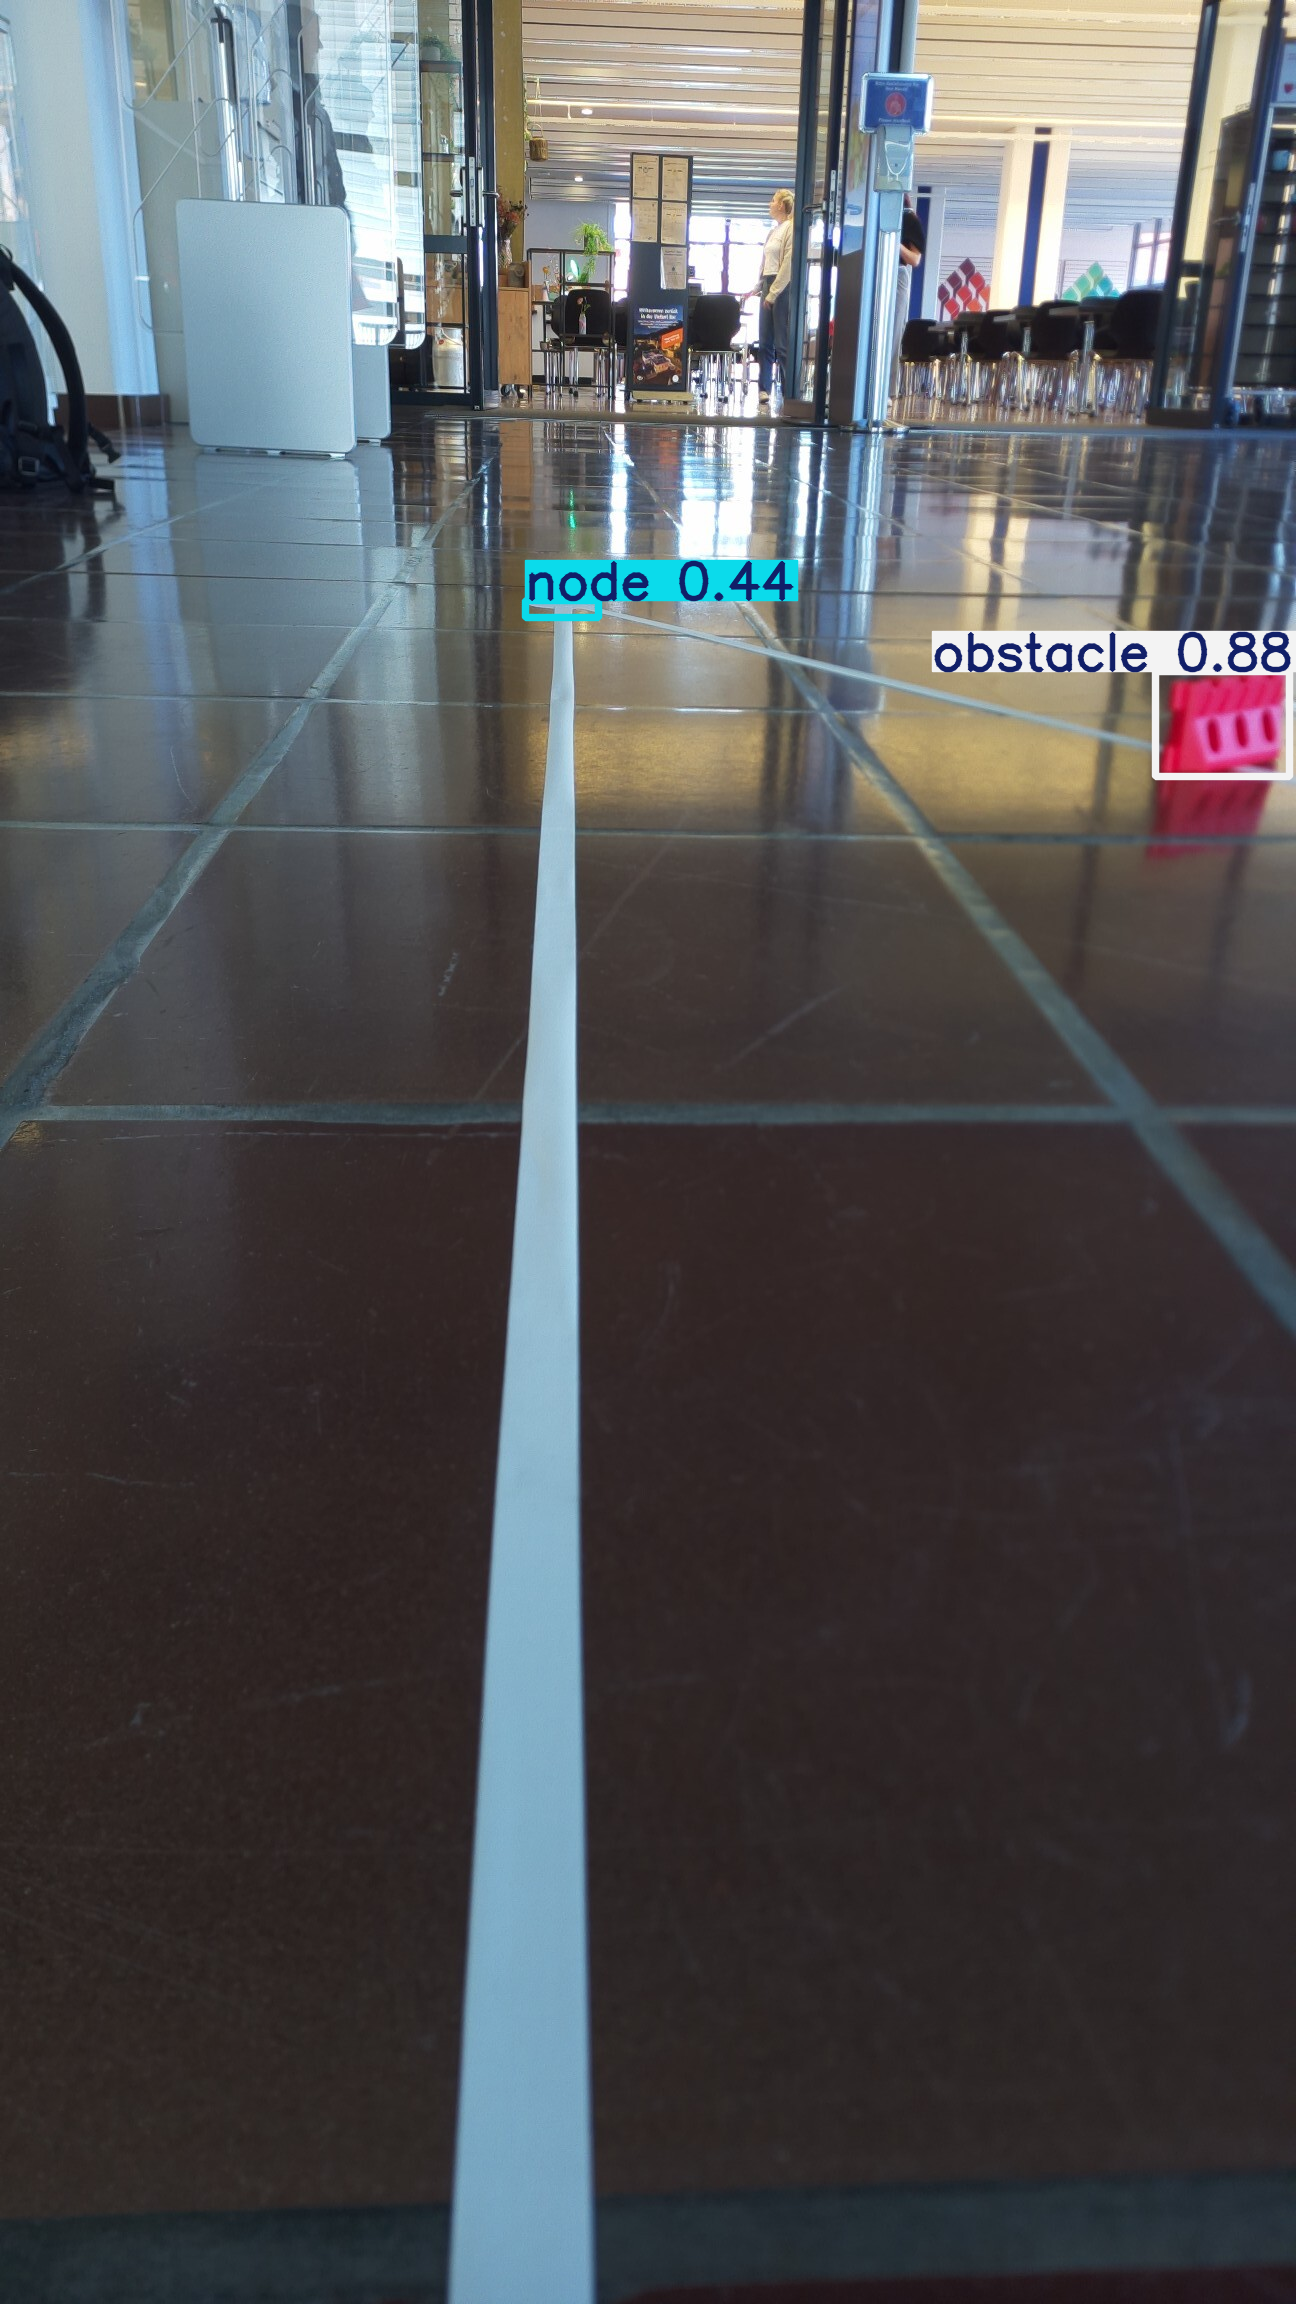
\includegraphics[width=\linewidth]{assets/IT/testing/yolo/node-obst-on-the-side_annot.png}
\end{minipage}
        &Knoten erkannt.&Knoten erkannt.& Erfüllt\\
  \hline


\end{tabularx}
\caption{Object Detector Testprotokoll}
\label{table:object-det-test}
\end{table}

Auf dem folgenden Bild \ref{img:object_detector_unittests} sind alle Unittests ersichtlich, die alle erfolgreich waren.

\begin{figure}[H]
\centering
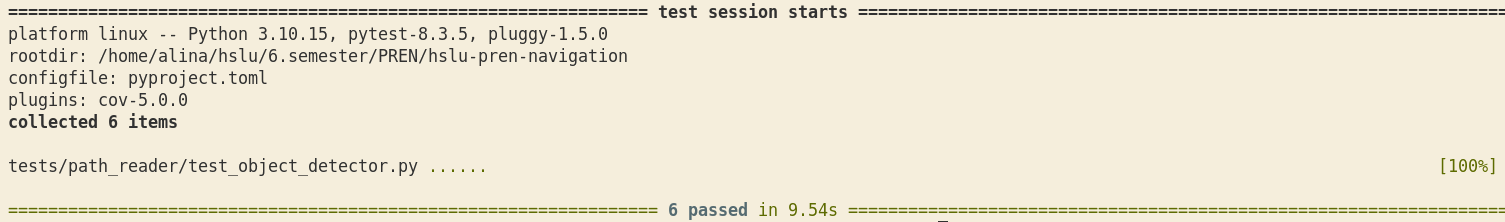
\includegraphics[width=\textwidth]{assets/IT/testing/yolo/object-detector-unittests.png}
\caption{Alle Object Detector Unittests}
\label{img:object_detector_unittests}
\end{figure}
%%%%%%%%%%%%%%%%%%%%%%% protocol opencv calibration %%%%%%%%%%%%%%%%%%%%%%%%


\includepdf[pages=-]{assets/IT/testing/protocol_opencv_calibration.pdf}


%%%%%%%%%%%%%%%%%%%%%%% testprocotol static node and edge detection %%%%%%%%%%%%%%%%%%%%%%%%

\includepdf[pages=-]{assets/IT/testing/testprotocol_static_node_edge_detection.pdf}